\documentclass[final,12pt]{colt2018} % Anonymized submission
%\usepackage{fullpage}
%\usepackage{amsthm}
\usepackage{amsmath}
\usepackage{amssymb}
\usepackage{algorithm}
\usepackage{algorithmic}
\usepackage[usenames,dvipsnames]{pstricks}
%\usepackage{epsfig}
\usepackage{pst-grad} % For gradients
\usepackage{pst-plot} % For axes
\usepackage{commath}
\usepackage{booktabs}

%\newtheorem{theorem}{Theorem}
%\newtheorem{lemma}{Lemma}
%\newtheorem{corollary}{Corollary}
\newtheorem{assumption}{Assumption}
\newtheorem{claim}{Claim}
%\newtheorem{definition}{Definition}

\renewcommand\algorithmicrequire{\textbf{input:}}
\renewcommand\algorithmicensure{\textbf{output:}}
\def\calF{\mathcal{F}}
\def\calG{\mathcal{G}}
\def\R{\mathbb{R}}
\def\E{\mathbb{E}}
\def\P{\mathbb{P}}
\def\calX{\mathcal{X}}
\def\calY{\mathcal{Y}}
\def\calH{\mathcal{H}}
\def\calO{\mathcal{O}}
\def\calA{\mathcal{A}}
\def\calW{\mathcal{W}}
\def\calZ{\mathcal{Z}}
\DeclareMathOperator{\argmin}{argmin}
\DeclareMathOperator{\B}{B}
\DeclareMathOperator{\HT}{P}
\DeclareMathOperator{\Alt}{Alt}
\DeclareMathOperator{\sign}{sign}
\DeclareMathOperator{\err}{err}
\DeclareMathOperator{\polylog}{polylog}
\DeclareMathOperator{\poly}{poly}
\def\Explore{\textsc{Explore}}
\def\Refine{\textsc{Refine}}

\def\cf{C_3}
\def\ct{C_5}
\def\ce{C_4}
\def\cs{C_6}
\def\cse{C_7}
\def\cfo{C_8}
\def\cn{C_9}

\title[Efficient active learning of sparse halfspaces]{Efficient active learning of sparse halfspaces}
\usepackage{times}

\coltauthor{\Name{Chicheng Zhang} \Email{chicheng.zhang@microsoft.com}
\\
\addr Microsoft Research \\
641 6th Avenue \\
New York, NY, 10011 \\
USA
}

\begin{document}

\maketitle

\begin{abstract}
We study the problem of efficient PAC active learning of homogeneous linear classifiers (halfspaces) in $\R^d$, where the goal is to learn
a halfspace with low error using as few label queries as possible.
Under the extra assumption that there is a $t$-sparse halfspace that
performs well on the data ($t \ll d$),
we would like our active learning algorithm to be {\em attribute efficient}, i.e. to have label requirements sublinear in $d$.
In this paper, we provide a computationally efficient algorithm that achieves this goal.
Under certain distributional assumptions on the data, our algorithm achieves a label complexity of $O(t \cdot \polylog(d, \frac 1 \epsilon))$.
In contrast, existing algorithms in this setting are either computationally inefficient, or subject to label requirements
polynomial in $d$ or $\frac 1 \epsilon$.
\end{abstract}
%In this setting, existing algorithms either achieve

%that the unlabeled distribution is log-concave, and the distribution satisfies

%While the non-sparse version of this problem is well studied, only a few works have made progress in
%this setting.
% !TeX root = main.tex
\section{Introduction}
\label{sec:intro}
Generative models are often trained in an unsupervised fashion, fitting a model $q$ to a set of observed data $x_P \subseteq X$ drawn iid from some true distribution $p$ on $x\in X$. Now, of course $p$ may not exactly belong to family $Q$ of probability distributions being fit, whether $Q$ consists of Gaussians mixture models, Markov models, or even neural networks of bounded size. We first discuss the limitations of generative modeling without feedback, and then discuss our model and results.

%\subsection{Limitations of Generative Modeling from Positive Examples Alone}
Consider fitting a generative model on a text corpus consisting partly of poetry written by four-year-olds and partly of mathematical publications from the {\em Annals of Mathematics}. Suppose that learning to generate a poem that looks like it was written by a child was easier than learning to generate a novel mathematical article with a correct, nontrivial statement. If the generative model pays a high price for generating unrealistic examples, then it may be better off learning to generate children's poetry than mathematical publications. However, without negative feedback, it may be difficult for a neural network or any other model to know that the mathematical articles it is generating are stylistically similar to the mathematical publications but do not contain valid proofs.\footnote{This is excluding clearly fake articles published without proper review in lower-tier venues \citep{LabbeL13}.} 

As a simpler example, the classic Markovian ``trigram model'' of natural language assigns each word a fixed probability conditioned only on the previous two words. Prior to recent advances in deep learning, for decades the trigram model and its variant were the workhorses of language modeling, assigning much greater likelihood to natural language corpora than numerous linguistically motivated grammars and other attempts \citep{Rosenfeld00}. However, text sampled from a trigram is typically nonsensical, e.g., the following text was randomly generated from a trigram model fit on a corpus of text from the Wall Street Journal \citep{JurafskyM09}:
\begin{quote}
They also point to ninety nine point six billion dollars from two hundred
four oh six three percent of the rates of interest stores as Mexico and
gram Brazil on market conditions. 
\end{quote}

In some applications, like text compression using a language model \citep{WittenNC87}, maximizing likelihood is equivalent to optimizing compression. However, in many  applications involving generation, such nonsense is costly and unacceptable. Now, of course it is possible to always generate valid data by returning random training examples, but this is simply overfitting and not learning. Alternatively, one could incorporate human-in-the-loop feedback such as through crowdsourcing, into the generative model to determine what is a valid, plausible sentence.

In some domains, validity could be determined automatically. Consider a Markovian model of a well-defined concept such as mathematical formulas that compile in \LaTeX{}. Now, consider a $n$-gram Markovian character model which the probability of each subsequent character is determined by the previous $n$ characters. For instance, the expression \$\{2+\{x-y\}\$ is invalid in \LaTeX{} due to mismatched braces. For this problem, a \LaTeX{} compiler may serve as a validity oracle. Various $n$-gram models can be fit which only generate valid formulas. To address mismatched braces, for example, one such model would ensure that it always closed braces within $n$ characters of opening, and had no nested braces. While an $n$-gram model will not perfectly model the true distribution over valid \LaTeX{} formulas, for certain generative purposes one may prefer an $n$-gram model that generates valid formulas over one that assigns greater likelihood to the training data but generates invalid formulas. 

Figure \ref{fig:rectangle} illustrates a simple case of learning a rectangle model for data which is not uniform over a rectangle. A maximum likelihood model would necessarily be the smallest rectangle containing all the data, but most examples generated from this distribution may be invalid. Instead a smaller rectangle, as illustrated in the figure, may be desired.

\begin{figure}[h]\label{fig:rectangle}
\centering
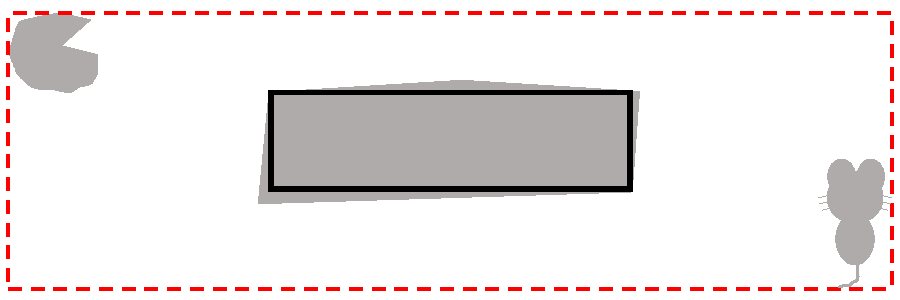
\includegraphics[width=3in]{fig.pdf}
\caption{Example where the underlying distribution $p$ is uniform over the (gray) valid regions. The solid rectangle maximizes our objective since it does not output nonsense (is supported only within the grey matter) and is closest to the $p$ (covers the maximum amount of grey matter). In contrast, the standard maximum likelihood (dashed red) rectangle must fully contain the observed samples, thus generating invalid points most of the time.  }
\end{figure}

Motivated by these observations, we evaluate a generative model $q$ on two axes. First is {\em coverage}, which is related to the probability assigned to future examples drawn from the true distribution $p$. Second is {\em validity}, defined as the probability that random examples generated from $q$ meet some validity requirement. Formally, we measure coverage in terms of a bounded {\em loss}:
$$\Loss(p,q)=\E_{x \sim p}[L(q_x)],$$
where $L:[0,1]\rightarrow [0,M]$ is a bounded decreasing function such as the capped log-loss $L(q_x)=\min(M, \log 1/q_x)$. % or $L(q_x)=\log 1/(q_x+\exp(-M))$. 
A bounded loss has the advantages of being efficiently estimable, and also it enables a model to assign 0 probability to one example (e.g., an outlier or error) if it greatly increases the likelihood of all other data. Validity is defined with respect to a set $V \subseteq X$, and $q(V)$ is the probability that a random example generated from $q$ lies within $V$. 

Clearly, there is a tradeoff between coverage and validity. We first focus on the case of (near) perfect validity. A Valid Generative Modeling (VGM) algorithm if it outputs, for a family of distributions $Q$ over $X$, if it outputs $\hat{q}$ with (nearly) perfect validity and whose loss is nearly as good as the loss of the best valid $q\in Q$. More precisely, $A$ is a VGM learner of $Q$ if for any nonempty valid subset $V \subseteq X$, any probability distribution $p$ over $V$, and any $\eps>0$, $A$ uses $n$ random samples from $p$ and makes $m$ membership oracle calls to $V$ and outputs a distribution $\hat{q}$ such that, $$\Loss(p, \hat{q}) \leq \min_{q \in Q: q(V)=1}\Loss(p,q) + \eps ~\text{ and }~\hat{q}(V)\geq 1-\eps.$$ 
We aim for our learner to be sample and query efficient, requiring that $n$ and $m$ are polynomial in $M, 1/\eps$ and a measure of complexity of our distribution class $Q$.
Furthermore, we would like our algorithms to be computationally efficient, with a runtime polynomial in the size of the data, namely the $n + m$ training examples. 
A more formal description of the problem is available in Section~\ref{sec:problem}.

$A$ is said to be {\em proper} if it always outputs $\hat{q}\in Q$ and {\em improper} otherwise.
In Section~\ref{sec:impossibility}, we first show that efficient proper learning for VGM is impossible. This is an information-theoretic result, meaning that even given infinite runtime and positive samples, one still cannot solve the VGM problem. Interestingly, this is different from binary classification, where it is possible to statistically learn from iid examples without a membership oracle.

Our first main positive result is an efficient (improper) learner for VGM. The algorithm relies on a subroutine that solves the following {\em Generative Modeling with Negatives} (GMN) problem: given sets $X_P, X_N \subset X$ of positive and negative examples, find the probability distribution $q \in Q$ which minimizes $\sum_{x \in X_P} L(q(x))$ subject to the constraint that $q(X_N)=0$. For simplicity, we present our algorithm for the case that the distribution family $Q$ is finite, giving sample and query complexity bounds that are logarithmic in terms of $|Q|$. However, as we show in Section~\ref{sec:infinite-families}, all of our results extend to infinite families $Q$. It follows that if one has a computationally efficient algorithm for the GMN problem for a distribution family $Q$, then our reduction gives a computationally efficient VGM learning algorithm for $Q$.

Our second positive result is an algorithm that minimizes $\Loss(p,q)$ subject to a relaxed validity constraint comparing against the optimal distribution that has validity $q(V)$ at least $1-\alpha$ for some $\alpha>0$. We show in Section~\ref{sec:partial-validity} that even in this more general setting, it is possible to obtain an algorithm that is statistically efficient but may not be computationally efficient. An important open question is whether there exists a computationally efficient algorithm for this problem when given access to an optimization oracle, as was the case for our algorithm for VGM.

\subsection{Related Work}
\cite{KearnsMRRSS94} showed how to learn distributions from positive examples in the realizable setting, i.e., where the true distribution is assumed to belong to the class being learned. In the same sense as their work is similar to PAC learning \citet{Valiant84} of distributions, our work is like agnostic learning \citet{KearnsSS94} in which no assumption on the true distribution is made. 

Generative Adversarial Networks (GANs)~\cite{GoodfellowPMXWOCB14} are an approach for generative modeling from positive examples alone, in which a generative model is trained against a discriminator that aims to distinguish real data from generated data. In some domains, GANs have been shown to outperform other methods at generating realistic-looking examples. Several shortcomings of GANs have been observed \citet{AroraRZ18}, and GANs are still subject to the theoretical limitations we argue are inherent to any model trained without a validity oracle. 

In supervised learning, there is a rich history of learning theory with various types of queries, including membership which are not unlike our (in)validity oracle. Under various assumptions, queries have been shown to facilitate the learning of complex classes such as finite automata \citet{Angluin88} and DNFs \citet{Jackson97}. See the survey of \cite{Angluin92} for further details.  Interestingly, \cite{Feldman09} has shown that for agnostic learning, i.e., without making assumptions on the generating distribution, the addition of membership queries does not enhance what is learnable beyond random examples alone. 
Supervised learning also has a large literature around active learning, showing how the ability to query examples reduces the sample complexity of many algorithms. See the survey of \cite{Hanneke14}. Note that the aim here is typically to save examples and not to expand what is learnable.
 
More sophisticated models, e.g., involving neural networks, can mitigate the invalidity problem as they often generate more realistic natural language and have even been demonstrated to generate \LaTeX{} that nearly compiles \citep{Karpathy15} or nearly valid Wikipedia markdown. However, longer strings generated are unlikely to be valid. For example, \cite{Karpathy15} shows generated markdown which includes:
\begin{quote}
==Access to ''rap===
The current history of the BGA has been [[Vatican Oriolean Diet]], British Armenian, published in 1893.  While actualistic such conditions such as the [[Style Mark Romanians]] are still nearly not the loss.
\end{quote}

Even ignoring the mismatched quotes and equal signs, note that this example has two so-called ``red links'' to two pages that do not exist. Without checking, it was not obvious to us whether or not Wikipedia had pages titled {\em Vatican Oriolean Diet} or {\em Style Mark Romanians}. In some applications, one may or may not want to disallow red links. In the case that they are considered valid, one may seek a full generative model of what might plausibly occur inside of brackets, as the neural network has learned in this case. If they are disallowed, a model might memorize links it has seen but not generate new ones. A validity oracle can help the learner identify what it should avoid generating.

 In practice, \cite{KusnerPH17} discuss how generative models from neural networks (in particular autoencoders) often generate invalid sequences. 
\cite{JanzWPKH18} learn the validity of examples output by a generative model using oracle feedback. 

\section{Related work}

%al
\paragraph{Attribute efficient active learning of halfspaces.}
There is a rich body of theoretical literature on active learning of general concept classes
in the PAC setting~\citep{D11, H14}. For the problem of active halfspace learning, sharp distribution-dependent label complexity results are known,
in terms of e.g. the splitting index~\citep{D05}, or the disagreement coefficient~\citep{H07}.
Direct applications of these results (without taking advantage of sparsity assumptions)
yield algorithms with label complexities at least $\Omega(d \ln \frac 1 \epsilon)$~\citep{KMT93}.
To make these algorithms attribute efficient, a natural modification is to consider concept class
$\calH_t$, the set of $t$-sparse linear classifiers.
It is well known that $\calH_t$ has VC dimension
$O(t \ln d)$. In conjunction with existing results in the active learning
literature, this observation immediately yields attribute efficient active
learning algorithms. For example, when the unlabeled distribution is isotropic log-concave,
an application of~\cite{ZC14}'s algorithm with $\calH_t$ yields a label complexity
of $O(t \ln d \ln \frac 1 \epsilon)$ in the $t$-sparse realizable setting, and gives
$O(t \ln d \cdot (\ln \frac 1 \epsilon+\frac{\nu^2}{\epsilon^2}))$ and
$O(\frac{t\ln d}{(1-2\eta)^2} \ln \frac 1 \epsilon)$
label complexities in the $t$-sparse $\nu$-adversarial noise and $t$-sparse $\eta$-bounded noise settings.\footnote{To see this, note that the $\phi(\cdot,\cdot)$ function
defined in~\cite{ZC14} with respect to $\calH_t$ can be bounded as: $\phi(r,\xi) \leq O(r \ln \frac{r}{\xi})$, as $\calH_t$ is a subset of $\calH$. Theorem 4 of \cite{ZC14} now applies.}
However, these algorithms require solving
empirical 0-1 loss minimization subject to sparsity constraints, which is computationally intractable in general~\citep{N95}.
The only attribute and computationally efficient PAC active learning algorithms we are aware of are in~\cite{ABHZ16}.  Specifically, under the $t$-sparse $\Omega(\epsilon)$-adversarial noise setting, \cite{ABHZ16} gives an efficient algorithm with label complexity $\tilde{O}(\frac{t}{\epsilon^2}\polylog(d,\frac 1 \epsilon))$. Under the $t$-sparse $\eta$-bounded noise setting, ~\cite{ABHZ16} gives an efficient algorithm with label complexity $\tilde{O}((\frac t \epsilon)^{O(\frac 1 {(1-2\eta)^2})})$.


%It is implicit in~\cite{D05} that the Splitting algorithm therein with input hypothesis
%class $\calH_t$ results in an inefficient algorithm
%with $\tilde O(t (\ln d + \ln \frac 1 \epsilon))$ label complexity in the $t$-sparse realizable setting.
%~\cite{H14} proposes an general splitting index based algorithm that


%efficient al
%For example, ~\cite{DKM05,BBZ07} achieves a label complexity of $O(d \ln \frac 1 \epsilon)$ in the realizable setting;
%~\cite{ABL17} achieves a label complexity of $\tilde{O}(d\ln \frac 1 \epsilon)$ in the $\nu$-adversarial noise setting, where $\nu = \Omega(\epsilon)$;
%~\cite{ABHU15} achieves a label complexity of $\tilde{O}(d\ln \frac 1 \epsilon)$ in the $\eta$-bounded noise setting, where $\eta$ is at most a constant.

%It combines the technique of margin-based active learning, polynomial regression~\cite{KKMS08} and $\ell_1/\ell_\infty$ Rademacher complexity bounds, and gives efficient algorithms with label complexity polynomial in $t$ and $\ln d$.

%On the other hand, many computationally efficient active halfspace learning algorithms have been proposed in the literature, with different degrees of noise tolerance~\cite{DKM05,BBZ07, ABL17, ABHU15, ABHZ16, YZ17}.
%However, all of the algorithms above have a label complexity at least $\Omega(d)$ and is thus not attribute efficient.

The notion of attribute efficient learning algorithms is initially studied in the pioneering works of~\cite{L87,B90}.
\cite{L87} considers attribute efficient online
learning of linear classifiers, with an application to learning disjunctions that depends on only $t$ attributes.
The algorithm incurs a mistake bound of $O(t \ln d)$, which can be of substantially lower order than $O(d)$ when $t$ is small.
\cite{B90} considers an online learning model where the feature space is infinite dimensional,
and each instance shown has a bounded number of nonzero attributes.
%In addition, there is an underlying concept that relies on
%only $t$ of the attributes.
It gives efficient algorithms that learn $k$-CNFs and disjunctions
with finite mistake bounds in this setting.
\cite{S00, KS06, STT12} study attribute efficient learning of decision lists and analyzes the
tradeoff between running time and mistake bound.
\cite{LS07} shows that, if the unlabeled distribution is unconcentrated over $\{-1,1\}^d$, then there
is an algorithm that learns $t$-sparse linear classifiers with a sample complexity of $\poly(t, \ln d, 2^{O(\epsilon^{-2})})$. \cite{F07} gives algorithms for attribute efficient learning parity and DNFs
in the membership query model.


%\cite{LS07} proposes an efficient algorithm that learns halfspaces
%over $t$ variables using $\poly(t, \ln d))$ samples to achieve a constant error.
%Winnow is attribute efficient, in the sense that
%when the instances and the classifiers are all $\ell_\infty$ bounded by a constant, and there is
%a $t$-sparse linear separator that separates the examples by a margin, then the mistake bound is
%$O(t \ln d)$, which only has a logarithmic dependence on the dimension.


\paragraph{One-bit compressed sensing.} The line of work on one-bit compressed sensing~\citep{BB08} is closely related to our problem setup. In this setting,
there is a unknown $t$-sparse vector $u \in \R^d$, and the algorithm can make measurements of $u$ using vectors $x \in \R^d$ and receives (possibly noisy) values of $\sign(u \cdot x)$.
Note that different from standard compressed sensing~\citep{CT06,D06}, the measurement results of one-bit compressed sensing are {\em quantized} versions of $(u \cdot x)$'s (i.e. they lie in $\{-1,+1\}$ as opposed to $\R$).
The goal is to approximately recover $u$ up to scaling with a few (ideally, $O(t \ln d)$) measurements.
 In the non-adaptive setting, the measurement vector
$x$'s are chosen at the beginning, while in the adaptive setting, the measurement vector $x$'s can be chosen sequentially,
based on past observations.
The problem of adaptive one-bit compressed sensing is therefore equivalent to attribute efficient
active halfspace learning in the membership query model~\citep{A88}.
We remark that active learning in the PAC model is more challenging than in the membership model, in that the learner has to query the labels of the unlabeled examples it has drawn.

%The crucial difference between the membership query model and the PAC model
%is that, in the PAC model, the , and is thus more challenging from the
%viewpoint of algorithm design.
%in the data
%stream literature
%This algorithm, in conjunction with
%a set of $O(\frac k \epsilon)$ nonadaptive Gaussian measurements, results in an nonadaptive 1-bit compressed sensing algorithm with
%$O(k (\ln d + \frac 1 \epsilon))$ measurements
%This, in conjunction with efficient noise tolerant learning algorithm
%working in the support of $w^*$, gives an algorithm that uses $O(k (\ln d + \frac{1}{(1-2\eta)^2 \epsilon})$ measurements.

~\cite{JLBB13} gives an algorithm that has robust recovery guarantees, however it is based on computationally-intractable $\ell_0$ minimization. Inspired by the count sketch data structure~\citep{CCF02}, ~\cite{HB11} proposes an efficient procedure that recovers the support of $u$ using $O(t \ln d)$ queries, and has strong noise tolerance properties. In conjunction with efficient full-dimensional active halfspace learning algorithms~\citep{DKM05,ABL17,CHK17,YZ17}, this procedure
 yields efficient algorithms that have label complexities of $O(t (\ln d + \ln \frac 1 \epsilon ))$
(resp. $O(t (\ln d + \ln \frac 1 \epsilon))$, $O(\frac{t}{(1-2\eta)^2} (\ln d + \ln \frac 1 \epsilon ))$) in the $t$-sparse realizable setting (resp. $t$-sparse $\Omega(\epsilon)$-adversarial noise setting, $t$-sparse $\eta$-bounded noise setting).
~\cite{GNJN13, ABK17} gives upper and lower bounds for {\em universal} one-bit compressed sensing, that is, the same set of measurements can be used to approximately recover {\em any} underlying $t$-sparse signal. In this setting,~\cite{ABK17} shows that, perhaps surprisingly, the number of measurements necessary and sufficient for support recovery is $\tilde{\Theta}(t^2 \ln d)$, as opposed to $\Theta(t \ln d)$ in the non-universal setting.
 ~\cite{PV13a} proposes a linear programming based algorithm that works in the $t$-sparse realizable setting, and has a measurement complexity of $\tilde{O}(\frac{t}{\epsilon^5})$,
based on a new tool named random hyperplane tessellations. ~\cite{L16} gives a support recovery algorithm that tolerates bounded noise, %double check this result - why don't they have a 1-2eta dependency?
using $\alpha$-stable random projections.
\cite{PV13b} proposes a convex programming based algorithm that works in the $t$-sparse $\Omega(\epsilon^2)$-adversarial noise model,
and has a measurement complexity of $\tilde{O}(\frac{t}{\epsilon^{12}})$.


Works on one-bit compressed sensing under the symmetric noise condition has been studied in the literature~\citep{PV13b, ZYJ14, CB15, ZG15}. In this model, it is assumed that there is a known function $g$, such that for all $x$, $\E[y|x] = g(u \cdot x)$. This assumption captures some realistic scenarios, but is nevertheless strong: it requires any two examples that have the same projection on $u$ to have the same conditional label distribution. In contrast, the $t$-sparse adversarial noise and the $t$-sparse bounded noise conditions allow heterogeneous noise levels, even among examples that have the same projection on $u$.
In this setting, the state of the art result of \cite{ZYJ14} gives an nonadaptive algorithm with $O(\frac{t \ln d}{ \epsilon^2})$. It also proposes an adaptive algorithm that works in same setting, achieving a label complexity bound of $O(\min(\frac{t \ln d}{\epsilon^2}, \frac{t\sqrt{d} \ln d}{\epsilon}))$, which is sometimes lower than that of the nonadaptive algorithm.
The special case of Gaussian noise before quantization has been studied extensively, i.e. given $x$, the label $y$ is generated by the formula $y = \sign(u \cdot x + n)$, where $n$ is a Gaussian random variable. \cite{GNR10} shows that when $u$ has a large dynamic range (the absolute value of the ratio between $u$'s largest and smallest nonzero elements in magnitude), adaptive approaches require fewer measurements to identify the support of $u$ than nonadaptive approaches.

%The most popular noise model is
%the generalized linear model, i.e. . The analysis crucially relies on the parameter $\lambda:=\E_{x \sim N(0,1)}[x g(x)]$; for example, $\lambda = \sqrt{\frac 2 \pi}(1 - 2\eta)$ when every label is flipped with probability $\eta$.
%\cite{PV13b} proposes a convex programming based algorithm that has a measurement complexity of $O(\frac{t \ln d}{\lambda^2 \epsilon^4})$. \cite{ZYJ14} gives a one-pass algorithm that has a measurement complexity of $O(\frac{t \ln d}{\lambda^2 \epsilon^2})$; see also \cite{ZG15} for refinements of logarithmic factors. \cite{CB15, ALPV14} studies
%subgaussian measurements; the recovery error bounds has an non-diminishing term under this general setting.
%depending on the Gaussianity of the measurements.
% whereas it tends to zero if the measurement distribution is sufficiently close to Gaussian.

%In classical compressed sensing, adaptive measurements have proven useful to reduce the measurement requirement~\cite{HBCN12}, or to reduce the signal to noise ratio requirement~\cite{MN14}. Similar results lie in 1-bit compressed sensing. ; \cite{ZYJ14} gives an adaptive algorithm that works in the parametric noise model, giving a measurement complexity of $O(\min(\frac{t \ln d}{\lambda^2\epsilon^2}, \frac{s\sqrt{d} \ln d}{\lambda^2\epsilon}))$, improving over the $O(\frac{t \ln d}{\lambda^2 \epsilon^2})$ bound in the nonadaptive setting.

%Attribute efficient active learning in the membership query model can be seen as an instance of adaptive one-bit compressed sensing.


%\cite{SSSHZ14} generalizes the analysis of \cite{L87}, and provide sample complexity bounds
%of order $\frac{t \ln d}{\epsilon^2}$ for ERM based algorithms.


%It proposes the Winnow algorithm, that achieves a mistake bound of $O(t \ln d)$ when the data is
%separable by a $t$-disjunction.
%the mistake bound has only a logarithmic dependence on the dimension of the data.




%achieving a mistake bound of
%$O(\frac{\|w^*\|_1^2 X^2 \ln d}{\gamma^2})$, under the assumption that the data is $\ell_\infty$ bounded by $X$,
%and is separable by $w^*$ with margin $\gamma$. Winnow is attribute efficient, in the sense
%that if $w^*$ is $t$-sparse and


% A straightforward application of~\cite{D05} yields an computationally inefficient algorithm that achieve a label
%complexity of $O(t (\ln d + \ln \frac 1 \epsilon))$ in this setting. On the other hand, if computational efficiency is
%required, the best known label complexity bounds are much worse, for instance, $O(\frac t {\epsilon^2})$~\cite{ABHZ16} and
%$O(d \ln \frac 1 \epsilon)$~\cite{DKM05, BBZ07}. As we will see in this note, we develop a computationally efficient algorithm that has a near-optimal label complexity
%bound of $O( t (\ln d)^3 \ln \frac 1 \epsilon )$, advancing the state of the art.
We provide a detailed comparison between our work and the results most closely related to ours in Tables~\ref{tab:comp-r}, \ref{tab:comp-an}, and \ref{tab:comp-bn}.



\begin{table}[t]
\centering
\begin{tabular}{llll}
\toprule
Algorithm & Model & Label complexity & Efficient? \\
\midrule
\begin{tabular}{@{}c@{}}\cite{HB11}\\ with \cite{DKM05} \end{tabular} & MQ & $\tilde{O}(t (\ln d + \ln \frac 1 \epsilon))$ & Yes \\
\cite{D05} & PAC & $\tilde{O}(t (\ln d + \ln \frac 1 \epsilon))$ & No \\
\cite{ABHZ16} & PAC & $\tilde{O}(\frac{t}{\epsilon^2} \polylog(d,\frac 1 \epsilon) )$ & Yes \\
Our work & PAC & $\tilde{O}(t \polylog(d,\frac 1 \epsilon) )$ & Yes \\
\bottomrule
\end{tabular}
\caption{A comparison of algorithms for active learning of halfspaces in the $t$-sparse realizable setting (Definition~\ref{def:r}); all the PAC algorithms above work under isotropic log-concave distributions.}
\label{tab:comp-r}
\end{table}


\begin{table}[t]
\centering
\begin{tabular}{lllll}
\toprule
Algorithm & Model & Noise tolerance  & Label complexity & Efficient? \\
\midrule
\begin{tabular}{@{}c@{}}\cite{HB11}\\ with \cite{ABL17} \end{tabular}& MQ & $\nu = \Omega(\epsilon)$ & $\tilde{O}(t (\ln d + \ln \frac 1 \epsilon))$ & Yes \\
\cite{ZC14} & PAC & $\nu = \Omega(\epsilon)$ & $\tilde{O}(t \ln d \ln \frac 1 \epsilon))$ & No \\
\cite{PV13b} & PAC  & $\nu = \Omega(\epsilon^2)$ & $\tilde{O}(\frac{t\ln d}{\epsilon^{12}})$ & Yes \\
\cite{ABHZ16} & PAC & $\nu = \Omega(\epsilon)$ & $\tilde{O}(\frac{t}{\epsilon^2} \polylog(d,\frac 1 \epsilon) )$ & Yes \\
Our work & PAC & $\nu = \Omega(\epsilon)$ & $\tilde{O}(t \polylog(d,\frac 1 \epsilon) )$ & Yes \\
\bottomrule
\end{tabular}
\caption{A comparison of algorithms for active learning of halfspaces in the $t$-sparse $\nu$-adversarial noise setting (Definition~\ref{def:an});  all the PAC algorithms above work under isotropic log-concave distributions.}
\label{tab:comp-an}
\end{table}

\begin{table}[t]
\centering
\begin{tabular}{lllll}
\toprule
Algorithm & Model & Noise tolerance & Label complexity & Efficient? \\
\midrule
\begin{tabular}{@{}c@{}}\cite{HB11}\\ with \cite{CHK17} \end{tabular} & MQ & $\eta \in [0,\frac 1 2)$ & $\tilde{O}(\frac{t}{(1-2\eta)^2} (\ln d + \ln \frac 1 \epsilon))$ & Yes \\
\cite{ZC14} & PAC & $\eta \in [0,\frac 1 2)$ & $\tilde{O}(\frac{t}{(1-2\eta)^2} \ln d \ln \frac 1 \epsilon))$ & No \\
\cite{ABHZ16} & PAC & $\eta \in [0,\frac 1 2)$ & $\tilde{O}((\frac{t}{\epsilon})^{O(\frac{1}{(1-2\eta)^2})} )$ & Yes \\
Our work & PAC & $\eta \in [0, \Omega(1))$ & $\tilde{O}(t \polylog(d,\frac 1 \epsilon) )$ & Yes \\
\bottomrule
\end{tabular}
\caption{A comparison of algorithms for active learning of halfspaces in the $t$-sparse $\eta$-bounded noise setting (Definition~\ref{def:bn}); all the PAC algorithms above work under isotropic log-concave distributions.}
\label{tab:comp-bn}
\end{table}

\section{Preliminaries}
We consider active learning in the PAC model~\citep{V84, KSS94}.
Denote by $\calX := \R^d$ the instance space, and $\calY := \{-1,+1\}$ the label space.
The learning algorithm is given a data distribution $D$ over $\calX \times \calY$. %, from which we can draw samples.
Denote by $D_X$ the marginal distribution of $D$ over $\calX$, and $D_{Y|X}$ the conditional distribution of label given instance.
%Throughout the paper, we assume that $D_X$ is isotropic log-concave.
The learning algorithm is also given a concept class, the set of homogeneous linear classifiers (halfspaces) $\calH:=\{\sign(w \cdot x): w \in \R^d \}$.
For any classifier $h: \calX \to \calY$, we denote by $\err(h):=\P_D(h(x) \neq y)$ the error rate of $h$.
Denote by $h^*$ the optimal classifier in $\calH$: $h^*:=\argmin_{h' \in \calH} \err(h')$.
The excess error of classifier $h$ is defined as $\err(h) - \err(h^*)$; in words, it is
the difference between $h$'s error and the best error in $\calH$. A vector $w$ corresponds to a
linear classifier $h_w := \sign(w \cdot x)$ whose decision boundary has $w$ as its normal; define $w^*$ as the unit vector $w$ such that $h_w = h^*$. We define the angle between two vectors $w, w'$ in $\R^d$ as $\theta(w,w') = \arccos(\frac{w \cdot w'}{\|w\|_2 \| w'\|_2})$. \cite{BL13} shows that there exist numerical constants $C_1, C_2 > 0$, such that if $D_X$ is isotropic log-concave, then for all $w, w'$ in $\R^d$,
\begin{equation}
 C_1 \P_D(h_w(x) \neq h_{w'}(x)) \leq \theta(w,w') \leq C_2 \P_D(h_w(x) \neq h_{w'}(x)).
\label{eqn:angdis}
\end{equation}

In active learning, the algorithm has the ability to draw unlabeled examples from $D_X$ and perform adaptive label queries to a labeling oracle $\calO$.
The oracle $\calO$ takes into input an unlabeled example $x$, and returns a label $y \sim D_{Y|X=x}$.
Given a random variable $z$ whose distribution is $\Delta$ over $\calZ$ and a set $T \subset \calZ$, denote by $\Delta|_T$ the conditional distribution of $z$ given that $z$ is in $T$.
An active learning algorithm is said to $(\epsilon,\delta)$-PAC
learn $\calH$ and $D$ with label complexity $n(\epsilon,\delta)$, if with probability $1-\delta$, it performs at most $n(\epsilon,\delta)$ label queries to $\calO$,
and returns a classifier $\hat{h}$ that has excess error at most $\epsilon$.

Given a vector $w$ and example $(x,y)$, the $\tau$-hinge loss $\ell_{\tau}(w, (x, y))$ is defined as $(1 - \frac{y w \cdot x}{\tau})_+$, where $(z)_+:=\max(0, z)$. Denote by $I(\cdot)$ the indicator function, that is, $I(A)$ is $1$ if predicate $A$ is true, is $0$ if $A$ is false.
A vector $v$ in $\R^d$ is said to be $s$-sparse, if it has at most $s$ nonzero entries.
For an integer $s \in \{1,2,\ldots,d\}$, define $\HT_s(\cdot)$ as the hard thresholding operation that takes a vector $v$ in $\R^d$ as input, and outputs a vector that keeps $v$'s $s$ largest entries in absolute value (breaking ties lexicographically), and setting all its other entries to zero~\citep{BD09}.
%Given a vector $w$ in $\R^d$ and $r>0$, denote by $\B_2(w,r):=\{w': \|w'-w\|_2 \leq r \}$ (resp. $\B_1(w,r)=\{w': \| w' - w \|_1 \leq r \}$) the $\ell_2$ (resp. $\ell_1$) ball centered at $w$ with radius $r$.

In this paper, we focus on the setting where there is a sparse halfspace that performs well under $D$.
Specifically, denote by $\calH_t := \{\sign(w \cdot x): w \in \R^d, \| w \|_0 \leq t \}$ the set of $t$-sparse halfspaces.
We consider the following two conditions on $D$:

%(at most $t$ of its
%entries are nonzero)
\begin{definition}
A distribution $D$ over $\calX \times \calY$ is said to satisfy the {\em $t$-sparse $\nu$-adversarial noise} condition for $\nu \in (0,1)$ and $t \in \{1,\ldots,d\}$, if there is a $t$-sparse unit vector $u$, such that $\P_D(\sign(u \cdot x) \neq y) \leq \nu$.
%\footnote{Note that $u$ may not be the optimal halfspace $w^*$, nevertheless, it can be seen by triangle inequality that $\theta(u,w^*) = O(\nu)$.}
\label{def:an}
\end{definition}
Observe that under this condition, $h_u$ is not necessarily the optimal classifier in $\calH$; in fact, it may not even be the optimal classifier in $\calH_t$. Nevertheless, by triangle inequality and Equation~\eqref{eqn:angdis}, the angle between $u$ and $w^*$ is at most $O(\nu)$.
It can be readily seen that if $t$ and $\nu$ are larger, the learning problem becomes more difficult. When $t = d$, the condition becomes the $\nu$-adversarial noise condition with respect to $\calH$~\citep{ABL17}.

\begin{definition}
A distribution $D$ over $\calX \times \calY$ is said to satisfy the {\em $t$-sparse $\eta$-bounded noise} condition for $\eta \in [0,\frac 1 2)$ and $t \in \{1,\ldots,d\}$, if there is a $t$-sparse unit vector $u$, such that
for every $x \in \calX$, $\P_D(\sign(u \cdot x) \neq y | x) \leq \eta$.
\label{def:bn}
\end{definition}
Under this condition, it can be seen that $h_u$ is the Bayes optimal classifier, therefore $u$ coincides with $w^*$.
It can be readily seen that if $t$ and $\eta$ are larger, the learning problem becomes more difficult. When $t = d$, the condition becomes the $\eta$-bounded noise condition with respect to $\calH$~\citep{MN06}.


%Note that the two conditions are incomparable: a distribution under the $\nu$ adversarial noise condition can have a region where the label flipping probability is
%close to $1/2$, while on the other hand, a distribution under the $b$-bounded noise condition can make any $t$-sparse classifier incur constant error.
Note that the above two conditions characterize different aspects of the data distribution $D$. The $t$-sparse $\nu$-adversarial noise condition only requires an upper bound on the total label flipping probability. On the other hand, the $t$-sparse $\eta$-bounded noise condition characterizes $D_{Y|X}$ everywhere in $\calX$: for every instance $x$, the expected label $\E[y|x]$ has the same sign as $u \cdot x$.
The following condition is a special case of the above two conditions by setting $\nu = 0$ or $\eta = 0$:

\begin{definition}
A distribution $D$ over $\calX \times \calY$ is said to satisfy the {\em $t$-sparse realizable} condition, for $t \in \{1,2,\ldots,d\}$, if there is a $t$-sparse unit vector $u$, such that $\P_D(\sign(u \cdot x) \neq y) = 0$.
\label{def:r}
\end{definition}

%Specifically, in passive learning, the algorithm
%is given $m$ labeled examples drawn iid from $D$, and returns a classifier $\hat{h}: X \to Y$.
%An algorithm is said to $(\epsilon,\delta)$-PAC learn $\calH$ and $D$ with sample complexity $m(\epsilon,\delta)$, if with probability $1-\delta$,
%it draws $m(\epsilon,\delta)$ labeled examples iid from $D$, and returns a classifier $\hat{h}$ that has excess error at most $\epsilon$.


%We study the problem of attribute-efficient active learning of linear separators.
%Suppose that the instances $x \in \R^d$ are drawn iid from an isotropic log-concave distribution over
%$\R^d$, and
% we are in the realizable case, where there is a targe linear separator $u$ such that $\| u \|_2 = 1$, and
% for all examples $(x,y)$ drawn, $y = \sign(u \cdot x)$.
% Our goal is to learn a linear separator $\hat{u}$ using active learning, using
%  as few label queries as possible. Existing active learning algorithms and lower bounds show a minimax label complexity of
%  $\Theta(d \ln \frac 1 \epsilon)$ for this problem.

  %that is,
  % we drawn unlabeled examples and perform label queries, such that the returned
  % $\hat{u}$ has angle at most $\epsilon$ to target $u$, with probability $1-\delta$,

%In this note, we focus on the setting that the target halfspace $u$ is {\em sparse}:
%\begin{assumption}[Sparse Target Halfspace]
%There are at most $t = o(d)$ nonzero entries of vector $u$.
%\end{assumption} Under the sparsity assumption,
%we hope to design computationally efficient algorithms that achieve better label complexites
%than the worst case $O(d \ln \frac 1 \epsilon)$ bound.

\section{Algorithm}
We present our main algorithm, namely Algorithm~\ref{alg:ae_al} in this section. We defer the exact settings of constants $c_1, c_2, c_3$ to Appendix~\ref{sec:params}.
Our algorithm uses the margin-based active learning framework, initially proposed by~\cite{BBZ07}.
Specifically, it proceeds in epochs, where at each epoch $k$, it draws a sample $S_k$ from distribution $D_X|_{B_k}$, queries their labels, and updates its iterate $w_k$ based on $S_k$. Due to technical reasons, at the first epoch ($k=0$), the sampling region $B_0$ and the constraint set $W_0$ are different from those in subsequent epochs. Throughout the process, the algorithm maintains the invariant that at each epoch $k$, $w_k$ is a  $t$-sparse unit vector.

At each epoch $k \geq 1$, the sampling region $B_k$ is a ``small-margin'' band $\{x: |w_{k-1} \cdot x| \leq b_k \}$, with bandwidth $b_k$ descreasing exponentially in $k$.
Then it performs constrained empirical hinge loss minimization over $S_k$, getting a linear classifier $w_k'$.
The constraint set $W_k$ is the intersection between an $\ell_1$ ball and an $\ell_2$ ball, centered at $w_{k-1}$ with different radii ($\rho_k$ and $r_k$). This is similar to the approach in~\cite{PV13b} for tackling the symmetric noise setting, where a linear optimization problem with a similar shaped constraint set is proposed. The construction of $W_k$'s is inspired by version space constructions in the PAC active learning literature~\citep{CAL94,BBL09,H14}.
Throughout the algorithm, we ensure $W_k$ to satisfy the following two properties with high probability: first, $u$ lie in all the $W_k$'s; second, the $W_k$'s are shrinking in size.\footnote{We refer the reader to Lemma~\ref{lem:induct} for a formal statement.}
In addition, the hinge loss used at epoch $k$ is parameterized by $\tau_k$, which also decreases exponentially in $k$.

Observe that $w_k'$ may not be a sparse vector; therefore, we perform a hard thresholding step (applying $\HT_t$), to ensure that our learned halfspace at the end of round $k$, is $t$-sparse. Hard thresholding has been widely used in the (unquantized) compressed sensing literature~\citep[See e.g.][]{BD09,GK09}, however its utility in one-bit compressed sensing is not yet well-understood. For example, ~\cite{JLBB13} proposes an algorithm named BIHT (binary iterative hard thresholding) that has strong empirical performance, but its convergence properties are unknown.
To the best of our knowledge, our work is the first that establishes convergence guarantees for iterative hard thresholding style algorithms for one-bit compressed sensing. We then perform a $\ell_2$ normalization step to ensure that our iterate $w_k$ is an unit vector, which has a scale comparable to $u$.

Finally, we remark that Algorithm~\ref{alg:ae_al} admits a computationally efficient implementation. First, the sampling regions $B_k$'s can be shown to have probability masses at least $\Omega(\epsilon)$ in $D_X$ for all $k$ in $\{0,1,\ldots,k_0\}$, which makes rejection sampling from $D_X|_{B_k}$ take $O(\frac 1 \epsilon)$ time per example.
Second, optimization problem~\eqref{eqn:opt} is convex, and can be approximately solved by e.g. stochastic gradient descent~\citep[See e.g.][Theorem 2]{SZ13} efficiently.

\begin{algorithm}[t]
  \caption{Attribute and computationally efficient active learning of halfspaces}
\begin{algorithmic}[1]
  \REQUIRE sparsity parameter $t$, target error $\epsilon$, failure probability $\delta$.
  \ENSURE  learned halfspace $\hat{w}$.
  \STATE Initialization: $k_0 \gets \lceil \log_2 \frac {1} {C_1 \epsilon} \rceil$, where $C_1$ is defined in Equation~\eqref{eqn:angdis}.
  \FOR{$k = 0, 1, 2 \ldots,k_0$}
  \STATE $S_k \gets $ sample $n_k = c_1 t (\ln d + \ln \frac{1}{\epsilon} + \ln\frac1{\delta_k})^3$ examples from $D_X|_{B_k}$ and query their labels, where
  \[ B_k := \begin{cases} \R^d, & k = 0, \\ \{x: |w_{k-1} \cdot x| \leq b_k \}, & k \geq 1, \end{cases}\]
	$\delta_k = \frac{\delta}{(k+1)(k+2)}$ and $b_k = c_2 \cdot 2^{-k}$.

  \STATE Solve the following optimization problem:
  \begin{equation}
    w_k' \gets \argmin_{w \in W_k} \sum_{(x,y) \in S_k} \ell_{\tau_k}(w, (x, y)),
    \label{eqn:opt}
  \end{equation}
  where
	%\B_2(0,1) \cap \B_1(0,\sqrt{t})
	%\B_2(w_{k-1},r_k) \cap \B_1(w_{k-1}, \rho_k)
  \[ W_k = \begin{cases} \{ w \in \R^d: \| w \|_2 \leq 1 \text{ and } \| w \|_1 \leq \sqrt{t} \}, & k = 0, \\ \{ w \in \R^d: \| w - w_{k-1} \|_2 \leq r_k \text{ and } \| w - w_{k-1} \|_1 \leq \rho_k \}, & k \geq 1, \end{cases}
  \]
  %\begin{cases}
  %\{w: \| w \|_2 \leq 1 \text{ and } \| w \|_1 \leq \sqrt{t} \}, & k = 0, \\
  %\{w: \| w - w_{k-1} \|_2 \leq r_k \text{ and } \| w - w_{k-1} \|_1 \leq \rho_k \}, & k \geq 1. \end{cases}
  $r_k = 2^{-k-3}$, $\rho_k = \sqrt{2t} \cdot 2^{-k-3}$, and $\tau_k = c_3 \cdot 2^{-k}$.
	\label{line:hlm}
  \STATE Let $w_k \gets \frac{\HT_t(w_k')}{\| \HT_t(w_k') \|_2}$.
	\label{line:ht}
  \ENDFOR
  \RETURN $w_{k_0}$.
\end{algorithmic}
\label{alg:ae_al}
\end{algorithm}

\section{Performance guarantees}

In this section, we prove Theorem~\ref{thm:main}, the main result of this paper. %for Algorithm~\ref{alg:ae_al}.
\begin{theorem}
  There exist numerical constants $\mu_1, \mu_2 \in (0, \frac 1 2)$ such that the following holds.
  Suppose $D_X$ is isotropic log-concave, and one of the following two conditions hold:
  \begin{enumerate}
    \item $D$ satisfies the $t$-sparse $\mu_1\epsilon$-adversarial noise condition;
    \item $D$ satisfies the $t$-sparse $\mu_2$-bounded noise condition.
  \end{enumerate}
	In addition, Algorithm~\ref{alg:ae_al} is run with sparsity parameter $t$, target error $\epsilon$ and failure probability $\delta$.
  Then, with probability $1-\delta$, the output halfspace $\hat{w}$ is such that
  $\err(h_{\hat{w}}) - \err(h^*) \leq \epsilon$,
  and the total number of label queries is $O( t \cdot (\ln d + \ln \frac 1 \epsilon)^3 \cdot \ln \frac 1 \epsilon )$.
  \label{thm:main}
\end{theorem}

As the $t$-sparse realizable setting is a special case of the $t$-sparse adversarial noise setting (by setting $\nu = 0$), Theorem~\ref{thm:main} immediately implies the
following corollary:
\begin{corollary}
	Suppose $D_X$ is isotropic log-concave, and the $t$-sparse realizable condition holds for $D$.
  In addition, Algorithm~\ref{alg:ae_al} is run with sparsity parameter $t$, target error $\epsilon$ and failure probability $\delta$.
  Then, with probability $1-\delta$, the output halfspace $\hat{w}$ is such that
  $\err(h_{\hat{w}}) - \err(h^*) \leq \epsilon$,
  and the total number of label queries is $O( t \cdot (\ln d + \ln \frac 1 \epsilon)^3 \cdot \ln \frac 1 \epsilon )$.
	\label{cor:main}
\end{corollary}
%We remark that although the requirement of $w_0$ seems strong, we can get an algorithm with the same label complexity
%unconditionally.
%Indeed, consider an arbitrary $t$-sparse unit vector $w_0 \in \R^d$; we run two copies of Algorithm~\ref{alg:ae_al}, initialized with $w_0$ and $-w_0$ respectively, getting classifiers $h_+$ and $h_-$. We can then run a standard hypothesis testing procedure to identify the classifier that has error guarantee $\epsilon$.
%This technique is well known in the literature; details can be found in (e.g.~\cite{ABL17}, Appendix B).

Theorem~\ref{thm:main} and Corollary~\ref{cor:main} imply that, under the respective noise conditions defined above, Algorithm~\ref{alg:ae_al}
has a label complexity of $O( t \polylog(d,  \frac 1 \epsilon) )$. To the best of our knowledge, this
is the first efficient PAC active learning algorithm that has a label complexity linear in $t$, and polylogarithmic
in $d$ and $\frac 1 \epsilon$. Previous works either need to sacrifice computational efficiency to achieve such guarantee~\citep{D05,ZC14}, or have label complexities polynomial in $d$ or $\frac 1 \epsilon$ ~\citep{ABL17, ABHZ16}. We remark that in the membership query model~\citep{A88, BB08}, efficient algorithms with $O( t \polylog(d,  \frac 1 \epsilon) )$ label complexities are implicit in the literature (e.g. by combining \cite{HB11}'s support recovery algorithm with efficient full-dimensional active halfspace learning algorithms~\citep{DKM05,ABL17,CHK17,YZ17}). In contrast, the focus of this paper is on the more challenging PAC setting, and it is unclear how to modify a membership query algorithm to make it work in the PAC setting.
%the membership query setting is harder than in the membership query setting.
%active learning in the PAC setting;


\subsection{Proof of Theorem~\ref{thm:main}}
Recall that $\delta_k = \frac{\delta}{(k+1)(k+2)}$; note that $\sum_{l=0}^{k_0} \delta_k \leq \delta$. To prove Theorem~\ref{thm:main}, we give exact settings of constants $\mu_1, \mu_2 \in (0, \frac 1 2)$ in Appendix~\ref{sec:params},
such that under either the $t$-sparse $\mu_1\epsilon$-adversarial noise condition or the $t$-sparse
$\mu_2$-bounded noise condition, the following lemma holds:
\begin{lemma}
	For every $k \in \{ 0,1,\ldots,k_0 \}$, there is an event $E_k$ with probability $1-\sum_{l=0}^k \delta_l$, on which $u$ is in $W_{k+1}$.
	%\B_1(w_k, \rho_{k+1}) \cap \B_2(w_k, r_{k+1})
	%$w_k$ is $t$-sparse, $\theta(w_k, u) \leq 2^{-k-3} \pi$ and $\| w_k - u \|_2 \leq 2^{-k-3} \pi$.
  %is t-sparse and
  %$\| w_{k-1} - u \|_2 \leq 2^{-k}$.
  \label{lem:induct}
\end{lemma}

The proof of Lemma~\ref{lem:induct} relies on the following two supporting lemmas. The first lemma (Lemma~\ref{lem:hlm}) shows that, $w_k'$ produced in the hinge loss minimization step (line~\ref{line:hlm}) has a small angle with $u$. Specifically, the upper bound on $\theta(w_k',u)$
is halved at each iteration $k$, with the help of constrained hinge loss minimization over a fresh set of $n_k = O(t \polylog(d,\frac1\epsilon))$ labeled examples. This relies on two ideas: first, as is standard
in the margin-based active learning framework~\citep[See e.g.][]{BBZ07,BL13}, it suffices to let $w_k'$ achieve a constant error with respect to the sampling distribution at epoch $k$; second, to ensure that the setting of $n_k$ ensures that $w_k'$ indeed has a constant error under the sampling distribution, we use a novel uniform concentration bound of hinge losses of $W_k$ over $S_k$ tighter than all prior works~\citep{ABL17,ABHZ16}. Thanks to our construction of $W_k$, our concentration bound of hinge losses is of order $\tilde{O}(\sqrt{\frac{t\ln d}{n_k}})$, which can be substantially tighter than
$\tilde{O}(\sqrt{\frac{d}{n_k}})$ used in~\citet{ABL17,HKY15} and $\tilde{O}(\sqrt{\frac{(t \ln d) \cdot 2^k}{n_k}})$ used in~\citet{ABHZ16}. We refer the reader to Appendix~\ref{sec:conc} for a formal statement.

 %in turn uses the generic results of~\cite{KST09} on the Rademacher complexity of $\ell_1$ bounded linear predictors.

%$w_{k-1}$ is t-sparse, $\theta(w_{k-1}, u) \leq 2^{-k-3} \pi$ and $\| w_{k-1} - u \|_2 \leq 2^{-k-3} \pi$
\begin{lemma}
For every $k \in \{ 0, 1,\ldots,k_0 \}$, if $u$ is in $W_k$, then with probability $1-\delta_k$, $\theta(w_k', u) \leq 2^{-k-8} \pi$.
\label{lem:hlm}
\end{lemma}

The second lemma (Lemma~\ref{lem:truncate}) shows that, performing a hard thresholding operation followed by $\ell_2$ normalization on $w_k'$ (line~\ref{line:ht}) yields a $t$-sparse unit vector $w_k$ that is close to $u$ in terms of both $\ell_1$ and $\ell_2$ distances. This ensures that $W_{k+1}$, the constraint set of the optimization problem at the next epoch, contains $u$. A key fact used in the proof of the lemma is that, the hard thresholding operator $\HT_t$ is effectively a $\ell_2$-projection onto the $\ell_0$ ball $\{w \in \R^d: \| w \|_0 \leq t \}$.


\begin{lemma}
For every $k \in \{ 0,1,\ldots,k_0 \}$, if $\theta(w_k', u) \leq 2^{-k-8} \pi$, then $u$ is in $W_{k+1}$.
\label{lem:truncate}
\end{lemma}
%then $w_k$ is $t$-sparse, $\| w_k - u \|_2 \leq 2^{-k-3} \pi$ and $\theta(w_k, u) \leq 2^{-k-3} \pi$

%The analysis of the first epoch (the base case $k=0$) is slightly different from the subsequent epochs, due to the usage of a different sampling region $B_1$ and constraint set $W_1$; this is taken care of by Lemma~\ref{lem:init} in the Appendix.

We are now ready to prove Lemma~\ref{lem:induct}.

\begin{proof}[Proof of Lemma~\ref{lem:induct}]
 We prove the lemma by induction.
\paragraph{Base case.} In the case of $k = 0$, observe that as $u$ has unit $\ell_2$ norm and $u$ is $t$-sparse, by Cauchy-Schwarz, $\| u \|_1 \leq \sqrt{t} \| u\|_2 = \sqrt{t}$. Therefore, $u$ belongs to the set $W_0$ deterministically.
Lemma~\ref{lem:hlm} with $k=0$ shows that there is an event $E_0$ with probability $1-\delta_0$, conditioned on which $\theta(w_0',u) \leq 2^{-8}\pi$. By Lemma~\ref{lem:truncate}, we get that $u$ is in $W_1$.
%$w_0$ is $t$-sparse, $\theta(w_0, w^*) \leq 2^{-3} \pi$ and $\| w_0 - w^* \|_2 \leq 2^{-3} \pi$.

% $w_{k-1}$ is $t$-sparse, $\theta(w_{k-1}, w^*) \leq 2^{-k-3} \pi$ and $\| w_{k-1} - w^* \|_2 \leq 2^{-k-3} \pi$
\paragraph{Inductive case.} For $k \geq 1$, suppose the inductive hypothesis holds. That is, there is an event $E_{k-1}$ with probability $1-\sum_{l=0}^{k-1} \delta_l$, such that
on $E_{k-1}$, $u$ is in $W_k$. By Lemma~\ref{lem:hlm}, there is an event $F_k$ such that $\P(F_k | E_{k-1}) \geq 1 - \delta_k$,
conditioned on which $\theta(w_k', u) \leq 2^{-k-8} \pi$.

%, with probability $1-\frac{\delta}{k(k+1)}$.

Define event $E_k:= E_{k-1} \cap F_k$. Observe that $\P(E_k) = \P(E_{k-1})\P(F_k | E_{k-1}) \geq 1-\sum_{l=0}^{k} \delta_l$.
%On event $E_k$, we have
Now, on event $E_k$, Lemma~\ref{lem:truncate} implies that $u$ is in $W_{k+1}$.
%$w_k$ is $t$-sparse, $\theta(w_k, w^*) \leq 2^{-k-3} \pi$ and $\| w_k - w^* \|_2 \leq 2^{-k-3} \pi$ holds.
This completes the induction.
\end{proof}

Theorem~\ref{thm:main} is now a direct consequence of Lemma~\ref{lem:induct}; we give its proof below.

\begin{proof}[Proof of Theorem~\ref{thm:main}]
From Lemma~\ref{lem:induct} and the fact that the output $\hat{w}$ is $w_{k_0}$, we have that with probability $1-\sum_{l=0}^{k_0}\delta_l \geq 1-\delta$, $u$ is in $W_{k_0+1}$. By the definition of $W_k$,
\[ \| u - w_{k_0} \|_2 \leq r_{k_0+1} = 2^{-k_0 - 4}. \]
By Lemma~\ref{lem:distangle} in the Appendix and the fact that $\|u\|_2 = 1$, we know that
$\theta(w_{k_0}, u) \leq \pi \| u - w_{k_0} \|_2 \leq 2^{-k_0 - 2} \leq \frac{C_1\epsilon}{2}$.
%$ \theta(\hat{w}, u) \leq 2^{-5} C_1 \epsilon.$
By the first inequality of Equation~\eqref{eqn:angdis}, we have that
$ \P_D (h_{w_{k_0}}(x) \neq h_{u}(x) ) \leq \frac \epsilon 2. $
Therefore, by triangle inequality and the fact that the output $\hat{w}$ is $w_{k_0}$,
\[ \err(h_{\hat{w}}) - \err(h_u) \leq \frac \epsilon 2. \]
We now consider two separate cases regarding the two different noise conditions:
\begin{enumerate}
\item In the $\mu_1 \epsilon$-adversarial noise setting, we know that $\err(h_u) \leq \mu_1 \epsilon \leq \frac \epsilon 2$.
Therefore,
\[ \err(h_{\hat{w}}) - \err(h^*) \leq \err(h_{\hat{w}}) \leq \err(h_u) + \frac \epsilon 2 \leq \frac \epsilon 2 + \frac \epsilon 2 \leq \epsilon. \]
\item In the $\mu_2$-bounded noise setting, as $h_u$ and $h^*$ are identical,
it immediately follows that $\err(h_{\hat{w}}) - \err(h^*) \leq \frac \epsilon 2 \leq \epsilon$.
\end{enumerate}

We now bound the label complexity of Algorithm~\ref{alg:ae_al}. The total number of labels queried is $\sum_{k=0}^{k_0} n_k$,
where $n_k \leq c_1 \cdot t (\ln d + \ln \frac 1 \epsilon + \ln \frac{k(k+1)}{\delta})^3$, and $k_0 = O(\ln\frac1\epsilon)$.
As a consequence, the total number of label queries is $O(t \cdot (\ln d + \ln \frac 1 \epsilon)^3 \cdot \ln \frac 1 \epsilon)$ in terms of $t, d$ and $\epsilon$.
The theorem follows.
\end{proof}


%Observe that Lemma 1 can be straightforwardly
%proved by induction in conjunction with the two claims.


%Now, denote by $S$ the support of $u$, $\hat{S}_k$ the set of coordinates that $P_t$ keeps on $\hat{w}_k'$.
%Additionally, for any vector $v$ and set $U \subset [d]$, denote by $v^U$ as the vector
%that agrees with $w$ on coordinates in $U$, and are 0's otherwise.
%We have that
%$\| \hat{w}_k'^{S^C} \|_2 = \| \hat{w}_k'^{S^C} - u^{S^C} \|_2 \leq \| \hat{w}_k' - u \|_2  \leq 2^{-k} / 4 $.
%By the optimality of $\hat{S}_k$,
%\[ \| \hat{w}_k'^{\hat{S}_k^C} \|_2 \leq \| \hat{w}_k'^{S^C} \|_2 \leq 2^{-k} / 4 \]
%Observe that $w_k = \hat{w}_k'^{\hat{S}_k^C}$, the above can be written as
%\[ \| \hat{w}_k' - w_k \|_2 \leq 2^{-k} / 4 \]
%Combining with Equation~\eqref{eqn:normalize_effect}, and triangle inequality, we have
%The lemma follows.
%\[ \| w_k - u \|_2 \leq \| \hat{w}_k' - w_k \|_2 + \| \hat{w}_k' - u \|_2 \leq 2^{-k} / 2. \]


\section{Conclusions}
%
We have investigated the setting of $d$-delayed composite anonymous feedback as applied to nonstochastic bandits. Composite anonymous feedback lends itself to formalize scenarios where the actions perfomed by the online decision maker produce long-lasting effects that combine additively over time. A general reduction technique was introduced that enables the convertion of a (backward stable) algorithm working in a standard bandit framework into one working in the composite feedback framework. 
In the case of $K$-armed bandits, we relied on a lower bound for bandit linear optimization in the probability simplex to show that no algorithm in the composite feedback framework can do better than $\scO(\sqrt{dKT})$. In turn, up to log factors, this is what we obtain as an upper bound by applying our reduction to the standard Exp3 algorithm.

We showed the generality and flexibility of our conversion technique by further applying it to Combinatorial Bandits (the Exp2 algorithm) and to Bandit Convex Optimization (the self-concordant barrier-based algorithms by \cite{ahr12} and \cite{st11}) with smooth/linear loss functions. In the latter case, the resulting Bandit Convex Optimization algorithm for composite anonymous feedback turned out to achieve regret bounds with higher rates than those of the corresponding base bandit algorithms, and we suspect that there is margin for improvement in our stability analysis of Lemma \ref{l:stabilityconvexscrible}.


\iffalse
************************
We then extended our results to the Bandit Convex Optimization framework, thereby showing the generality and flexibility of our conversion technique. As an example, we applied 

We Our reduction is flexible

 that works under the assumption of an oblivious adversary generating loss components. 

provided a general reduction that does such and such

in the case of k armed upper and lower bound, matching up to log factors. lower bound reduces to bandit linear optimization




flexibility, extension to combinatorial and bco, an example of application with beta smooth and self-concordant barriers.

Our analysis of bco is almost certainly suboptimal,
************************
\fi




\section*{Acknowledgments}
I am grateful to Daniel Hsu for suggesting this research direction to me, and many insightful discussions along this line. I would also like to thank Pranjal Awasthi, Jie Shen and Hongyang Zhang for helpful initial conversations about the results in this paper. I thank the anonymous COLT reviewers for their thoughtful comments. Special thanks to Yue Liu, who provided unconditional support throughout this research project.

%\bibliographystyle{plain}
\bibliography{alsearch}

 %Oftentimes we assume that
 %$u^*$ is sparse, that is, there are at most $k$ nonzero elements ($k \ll d$) in vector $u$.
\newpage
\appendix
\appendix

\section{Proof of Lemma \ref{thm:general_instantaneous}}
\begin{proof}{\textbf{of Lemma \ref{thm:general_instantaneous}}.}
We first state a useful property used in typical OMD analysis. Let $\Omega$ be a convex compact set in $\mathbb{R}^K$, $\psi$ be a convex function on $\Omega$, 
$w'$ be an arbitrary point in $\Omega$, and $x \in \mathbb{R}^K$.
If $w^*=\argmin_{w\in \Omega}\{\inn{w,x}+D_{\psi}(w,w')\}$, then for any $u \in \Omega$,
\begin{align*}
\inn{w^*-u, x}\leq D_{\psi}(u,w')-D_\psi(u,w^*)-D_{\psi}(w^*,w'). 
\end{align*}
This is by the first-order optimality condition of $w^*$ and direct calculations. Applying this to update rule~\eqref{eqn:update_rule_2} we have
\begin{align}
\inn{w_{t+1}^\p-u, \hat{\ell}_t+ a_t} \leq D_{\psi_t}(u,w_{t}^\p)-D_{\psi_t}(u,w_{t+1}^\p)-D_{\psi_t}(w_{t+1}^\p, w_{t}^\p); \label{eqn:apply1}
\end{align}
while applying it to update rule~\eqref{eqn:update_rule_1} and picking $u=w_{t+1}^\p$ we have
\begin{align}
\inn{w_t-w_{t+1}^\p, m_t} \leq D_{\psi_t}(w_{t+1}^\p, w_t^\p)-D_{\psi_t}(w_{t+1}^\p, w_t)-D_{\psi_t}(w_t, w_t^\p).\label{eqn:apply2} 
\end{align}
Now we bound the instantaneous regret as follows:
\begin{align}
&\inn{w_t-u, \hat{\ell}_t}\nonumber \\
&=\inn{w_t-u, \hat{\ell}_t+ a_t}-\inn{w_t, a_t}+\inn{u,  a_t}\nonumber \\
&=\inn{w_t-w_{t+1}^\p, \hat{\ell}_t+a_t}-\inn{w_t, a_t}+\inn{w_{t+1}^\p-u, \hat{\ell}_t+a_t}+\inn{u,   a_t}\nonumber \\
&=\inn{w_t-w_{t+1}^\p, \hat{\ell}_t+a_t-m_t}-\inn{w_t,a_t}+\inn{w_{t+1}^\p-u, \hat{\ell}_t+ a_t}+\inn{w_t-w_{t+1}^\p, m_t}+\inn{u,   a_t} \nonumber \\
&\leq D_{\psi_t}(u,w_{t}^\p)-D_{\psi_t}(u,w_{t+1}^\p)-D_{\psi_t}(w_{t+1}^\p, w_t)-D_{\psi_t}(w_t, w_t^\p)+\inn{u, a_t}, \label{eqn:regret_decomposition}
\end{align}
where last inequality is by the condition $\inn{w_t-w_{t+1}^\p, \hat{\ell}_t+a_t-m_t}-\inn{w_t,a_t}\leq 0$, Eq.~\eqref{eqn:apply1}, and Eq.~\eqref{eqn:apply2}.
\end{proof}

\section{Lemmas for Log-barrier OMD}
\label{section:all_kinds_of_lemmas}

In this section we establish some useful lemmas for update rules~\eqref{eqn:update_rule_1} and~\eqref{eqn:update_rule_2} with log-barrier regularizer,
which are used in the proofs of other theorems.
We start with some definitions.

\begin{definition}
\label{definition:norm}
For any $h \in \mathbb{R}^K$, define norm $\norm{h}_{t,w}=\sqrt{h^\top \nabla^2 \psi_t(w) h}=\sqrt{\sum_{i=1}^K \frac{1}{\eta_{t,i}}\frac{h_i^2}{w_i^2}}$ and its dual norm $\norm{h}_{t,w}^*=\sqrt{h^\top \nabla^{-2} \psi_t(w) h}=\sqrt{\sum_{i=1}^K \eta_{t,i}w_i^2 h_i^2}$.
For some radius $r > 0$, define ellipsoid $\mathcal{E}_{t,w}(r)=\left\{u \in \mathbb{R}^K : \norm{u-w}_{t,w}\leq r \right\}$ . 
\end{definition}

\begin{lemma}
\label{lemma:norm_close}
If $w^\p \in \mathcal{E}_{t,w}(1)$ and $\eta_{t,i}\leq \frac{1}{81}$ for all $i$, then $w_i^\p\in \left[ \frac{1}{2}w_i, \frac{3}{2}w_i \right]$ for all $i$, and also $ 0.9\norm{h}_{t,w} \leq \norm{h}_{t,w^\p} \leq 1.2\norm{h}_{t,w}$ for any $h\in \mathbb{R}^K$. 
\end{lemma}
\begin{proof}
$w^\p\in \mathcal{E}_{t,w}(1)$ implies $\sum_{i=1}^K \frac{1}{\eta_{t,i}}\frac{(w^\p_i-w_i)^2}{w_i^2}\leq 1$. Thus for every $i$, we have $\frac{\abs{w_i^\p-w_i}}{w_i}\leq \sqrt{\eta_{t,i}}\leq \frac{1}{9}$, implying $w_i^\p\in \left[ \frac{8}{9}w_i, \frac{10}{9}w_i \right]\subset\left[ \frac{1}{2}w_i, \frac{3}{2}w_i \right]$. 
Therefore, $\norm{h}_{t,w^\p}
=\sqrt{\sum_{i=1}^K \frac{1}{\eta_{t,i}} \frac{h_i^2}{w^{\p 2}_i}}
\geq \sqrt{\sum_{i=1}^K \frac{1}{\eta_{t,i}}\frac{h_i^2}{\left(\frac{10}{9}w_i\right)^2}}
=0.9\norm{h}_{t,w}$. 
Similarly, we have $\norm{h}_{t,w^\p}\leq 1.2\norm{h}_{t,w}$. 
\end{proof}

\begin{lemma}
\label{lemma:stability}
Let $w_t, w_{t+1}^\p$ follow \eqref{eqn:update_rule_1} and \eqref{eqn:update_rule_2} where $\psi_t$ is the log-barrier with $\eta_{t,i}\leq \frac{1}{81}$ for all $i$. If $\norm{\hat{\ell}_t-m_t+a_t}^*_{t,w_t}\leq \frac{1}{3}$, then $w_{t+1}^\p \in \mathcal{E}_{t,w_t}(1)$. 
\end{lemma}

\begin{proof}
Define $F_{t}(w)=\inn{w, m_t}+D_{\psi_t}(w, w_t^\p)$ and $F_{t+1}^\p(w)=\inn{w, \hat{\ell}_t+a_t}+D_{\psi_t}(w, w_t^\p)$. Then by definition we have $w_t=\argmin_{w\in\Omega}F_{t}(w)$ and $w_{t+1}^\p=\argmin_{w\in\Omega}F_{t+1}^\p(w)$. To show $w_{t+1}^\p\in \mathcal{E}_{t,w_t}(1)$, it suffices to show that for all $u$ on the boundary of $\mathcal{E}_{t,w_t}(1)$, $F^\p_{t+1}(u)\geq F^\p_{t+1}(w_t)$. 

Indeed, using Taylor's theorem, for any $u\in \partial \mathcal{E}_{t,w_t}(1)$, there is an $\xi$ on the line segment between $w_t$ and $u$ such that (let $h\triangleq u-w_t$)
\begin{align*}
F^\p_{t+1}(u)&=F^\p_{t+1}(w_t)+\nabla F^{\p}_{t+1} (w_t)^\top h+ \frac{1}{2}h^\top\nabla^2 F^\p_{t+1}(\xi)h \\
&=F^\p_{t+1}(w_t)+ (\hat{\ell}_t-m_t+a_t)^\top h +\nabla F_t (w_t)^\top h+ \frac{1}{2}h^\top\nabla^2 \psi_t(\xi)h \\
&\geq F^\p_{t+1}(w_t)+ (\hat{\ell}_t-m_t+a_t)^\top h + \frac{1}{2}\norm{h}_{t,\xi}^2 \tag{by the optimality of $w_t$}\\
&\geq F^\p_{t+1}(w_t)+ (\hat{\ell}_t-m_t+a_t)^\top h + \frac{1}{2}\times0.9^2\norm{h}_{t,w_t}^2 \tag{by Lemma \ref{lemma:norm_close}} \\
&\geq F^\p_{t+1}(w_t)- \norm{\hat{\ell}_t-m_t+a_t}^*_{t,w_t} \norm{h}_{t,w_t} + \frac{1}{3}\norm{h}_{t,w_t}^2 \\
&=F^\p_{t+1}(w_t)- \norm{\hat{\ell}_t-m_t+a_t}^*_{t,w_t} + \frac{1}{3} \tag{$\norm{h}_{t,w_t}=1$}\\
&\geq F^\p_{t+1}(w_t). \tag{by the assumption}
\end{align*}
\end{proof}

\begin{lemma}
\label{lemma:stability_under_condition}
Let $w_t, w_{t+1}^\p$ follow \eqref{eqn:update_rule_1} and \eqref{eqn:update_rule_2} where $\psi_t$ is the log-barrier with $\eta_{t,i}\leq \frac{1}{81}$ for all $i$. If $\norm{\hat{\ell}_t-m_t+a_t}^*_{t,w_t}\leq \frac{1}{3}$, then $\norm{w_{t+1}^\p-w_t}_{t,w_t}\leq 3\norm{\hat{\ell}_t-m_t+a_t}_{t,w_t}^*$. 
\end{lemma}
\begin{proof}
Define $F_t(w)$ and $F_{t+1}^\p(w)$ to be the same as in Lemma \ref{lemma:stability}. Then we have 
\begin{align}
F_{t+1}^\p(w_t)-F_{t+1}^\p(w_{t+1}^\p)&=(w_t-w_{t+1}^\p)^\top(\hat{\ell}_t-m_t+a_t) + F_t(w_t)-F_t(w_{t+1}^\p) \nonumber \\
&\leq (w_t-w_{t+1}^\p)^\top(\hat{\ell}_t-m_t+a_t) \nonumber \tag{optimality of $w_t$}\\
&\leq \norm{w_t-w_{t+1}^\p}_{t,w_t}\norm{\hat{\ell}_t-m_t+a_t}_{t,w_t}^*. \label{eqn:direction1}
\end{align}
On the other hand, for some $\xi$ on the line segment between $w_t$ and $w_{t+1}^\p$, we have by Taylor's theorem and the optimality of $w_{t+1}^\p$,
\begin{align}
F_{t+1}^\p(w_t)-F_{t+1}^\p(w_{t+1}^\p)&=\nabla F_{t+1}^\p(w_{t+1}^\p)^\top (w_t-w_{t+1}^\p) + \frac{1}{2}(w_t-w_{t+1}^\p)^\top \nabla^2 F_{t+1}^\p(\xi)(w_t-w_{t+1}^\p) \nonumber \\
&\geq \frac{1}{2}\norm{w_t-w_{t+1}^\p}_{t,\xi}^2 .
\label{eqn:direction2}
\end{align}
Since the condition in Lemma \ref{lemma:stability} holds, $w_{t+1}^\p\in \mathcal{E}_{t,w_t}(1)$, and thus $\xi\in \mathcal{E}_{t,w_t}(1)$. Using again Lemma \ref{lemma:norm_close}, we have 
\begin{align}
\frac{1}{2}\norm{w_t-w_{t+1}^\p}_{t,\xi}^2 \geq \frac{1}{3}\norm{w_t-w_{t+1}^\p}_{t,w_t}^2\label{eqn:direction3}.
\end{align}
Combining \eqref{eqn:direction1}, \eqref{eqn:direction2}, and \eqref{eqn:direction3}, we have $\norm{w_t-w_{t+1}^\p}_{t,w_t}\norm{\hat{\ell}_t-m_t+a_t}_{t,w_t}^* \geq \frac{1}{3}\norm{w_t-w_{t+1}^\p}_{t,w_t}^2$, which leads to the stated inequality. 
\end{proof}

\begin{lemma}
\label{lemma:condition_automatic_hold}
%Let $w_t, w_{t+1}^\p$ follow \eqref{eqn:update_rule_1} and \eqref{eqn:update_rule_2}. 
When the three conditions in Theorem \ref{lemma:MAB_condition} hold, we have $\norm{\hat{\ell}_t-m_t+a_t}^{*}_{t,w_t}\leq \frac{1}{3}$ for either $a_{t,i}=6\eta_{t,i}w_{t,i}(\hat{\ell}_{t,i}-m_{t,i})^2$ or $a_{t,i}=0$.  
\end{lemma}
\begin{proof}
For $a_{t,i}=6\eta_{t,i}w_{t,i}(\hat{\ell}_{t,i}-m_{t,i})^2$, we have
\begin{align*}
\norm{\hat{\ell}_t-m_t+a_t}^{*2}_{t,w_t}
&= \sum_{i=1}^K\eta_{t,i}w_{t,i}^2\big(\hat{\ell}_{t,i}-m_{t,i} + 6\eta_{t,i}w_{t,i}(\hat{\ell}_{t,i}-m_{t,i})^2\big)^2 \\
&=\sum_{i=1}^K\eta_{t,i}w_{t,i}^2(\hat{\ell}_{t,i}-m_{t,i})^2+12\eta_{t,i}^2w_{t,i}^3(\hat{\ell}_{t,i}-m_{t,i})^3 +36\eta_{t,i}^3w_{t,i}^4(\hat{\ell}_{t,i}-m_{t,i})^4\\
&\leq \sum_{i=1}^K \eta_{t,i}w_{t,i}^2(\hat{\ell}_{t,i}-m_{t,i})^2(1+36\eta_{t,i}+324\eta_{t,i}^2) \tag{condition (ii)}\\
&\leq 2\sum_{i=1}^K \eta_{t,i}w_{t,i}^2(\hat{\ell}_{t,i}-m_{t,i})^2 \tag{condition (i)}\\
&\leq 2\times \frac{1}{18}=\frac{1}{9}.\tag{condition (iii)}
\end{align*}
For $a_{t,i}=0$, we have
\begin{align*}
\norm{\hat{\ell}_t-m_t+a_t}^{*2}_{t,w_t}=\norm{\hat{\ell}_t-m_t}^{*2}_{t,w_t}=\sum_{i=1}^K \eta_{t,i}w_{t,i}^2(\hat{\ell}_{t,i}-m_{t,i})^2\leq \frac{1}{18} < \frac{1}{9}. \tag{condition (iii)}
\end{align*}
%When $a_{t,i}=0$,
%\begin{align*}
%\norm{\hat{\ell}_t-m_t+a_t}_{t,w_t}^{*2}= \sum_{i=1}^K \eta_{t,i}w_{t,i}^2(\hat{\ell}_{t,i}-m_{t,i})^2 \leq \frac{1}{18}<\frac{1}{9}. \text{\ \ \ \ \ \ \ \ \ \ \ \ \ \ \ \ \ \ \ \ \ \ \ (condition(iii))} 
%\end{align*}
\end{proof}

\begin{lemma}
\label{lemma:2times_bound}
If the three conditions in Theorem \ref{lemma:MAB_condition} hold, \textsc{Broad-OMD} (with either Option I or II)
satisfies $\frac{1}{2}w_{t,i}\leq w^\p_{t+1,i}\leq \frac{3}{2}w_{t,i}$.
%Let $w_t, w_{t+1}^\p$ follow \eqref{eqn:update_rule_1} and \eqref{eqn:update_rule_2}. If the three conditions in Theorem \ref{lemma:MAB_condition} hold, then $\frac{1}{2}w_{t,i}\leq w^\p_{t+1,i}\leq \frac{3}{2}w_{t,i}$, for either $a_{t,i}=6\eta_{t,i}w_{t,i}(\hat{\ell}_{t,i}-m_{t,i})^2$ or $a_{t,i}=0$.
\end{lemma}
\begin{proof}
This is a direct application of Lemmas \ref{lemma:condition_automatic_hold},  \ref{lemma:stability}, and \ref{lemma:norm_close}.
%It suffices to prove $w_{t+1}^\p \in \mathcal{E}_{t,w_t}(1)$, because if it is true, then
%\begin{align*}
%\norm{w_{t+1}^\p-w_t}_{t,w_t}=\sqrt{\sum_{i=1}^K\frac{1}{\eta_{t,i}}\frac{(w^\p_{t+1,i}-w_{t,i})^2}{w_{t,i}^2}}\leq 1, 
%\end{align*}
%which implies $\frac{\abs{w_{t+1,i}^\p-w_{t,i}}}{w_{t,i}}\leq \sqrt{\eta_{t,i}}\leq \frac{1}{2}$. Thus, $w_{t+1,i}^\p \in [\frac{1}{2}w_{t,i}, \frac{3}{2}w_{t,i}]$.

%Since we assume the three conditions in Theorem \ref{lemma:MAB_condition} hold, $w_{t+1}^\p \in \mathcal{E}_{t,w_t}(1)$ can be proved by applying Lemma \ref{lemma:condition_automatic_hold} and Lemma \ref{lemma:stability} back to back.

\end{proof}

\begin{lemma}
\label{lemma:2times_bound_another}
For the MAB problem, if the three conditions in Theorem \ref{lemma:MAB_condition} hold, \textsc{Broad-OMD} (with either Option I or II)
satisfies $\frac{1}{2}w_{t,i}\leq w^\p_{t,i}\leq \frac{3}{2}w_{t,i}$.
\end{lemma}
\begin{proof}
It suffices to prove $w_{t}^\p \in \mathcal{E}_{t,w_t}(1)$ by Lemma~\ref{lemma:norm_close}.
Since we assume that the three conditions in Theorem \ref{lemma:MAB_condition} hold and $w_t\in \Delta_K$, we have $\norm{m_t}_{t,w_t}^*=\sqrt{\sum_{i=1}^K \eta_{t,i}w_{t,i}^2m_{t,i}^2}\leq \sqrt{\frac{1}{162}\sum_{i=1}^K w_{t,i}^2}\leq \sqrt{\frac{1}{162}}< \frac{1}{3}$. This implies $w_{t}^\p \in \mathcal{E}_{t,w_t}(1)$ by a similar arguments as in the proof of Lemma~\ref{lemma:stability} (one only needs to replace $F_{t+1}^\p(w)$ there by $G(w)\triangleq D_{\psi_t}(w,w_t^\p)$ and note that $w_t^\p=\argmin_{w\in \Delta_K}G(w)$).
\end{proof}


%\begin{lemma}
%\label{lemma:stability_game}
%For MAB problems, if the three conditions in Theorem \ref{lemma:MAB_condition} hold, then \textsc{Broad-OMD} with $a_{t,i}=\mathbf{0}$ and fixed learning rate $\eta$ guarantees $\norm{w_{t+1}-w_t}_1 = \mathcal{O}(\eta)$ for all $t$.  
%\end{lemma}
%\begin{proof}
%By Lemma \ref{lemma:condition_automatic_hold} and \ref{lemma:stability_under_condition}, we have $\norm{w_t-w_{t+1}^\p}_{t,w_t}\leq 3\norm{\hat{\ell}_t-m_t}_{t,w_t}^*$, which implies
%\begin{align*}
%\frac{1}{\eta}\frac{(w_{t,j}-w_{t+1,j}^\p)^2}{w_{t,j}^2}\leq \sum_{i=1}^K\frac{1}{\eta}\frac{(w_{t,i}-w_{t+1,i}^\p)^2}{w_{t,i}^2}\leq 3\eta\sum_{i=1}^K  w_{t,i}^2(\hat{\ell}_{t,i}-m_{t,i})^2\leq 3\eta\times 9. 
%\end{align*}
%Therefore, $\abs{w_{t,j}-w_{t+1,j}^\p} = \mathcal{O}(\eta w_{t,j})$. We can use similar techniques in Lemma \ref{lemma:condition_automatic_hold} and \ref{lemma:stability_under_condition} to prove $\norm{w_{t+1}-w_{t+1}^\p}_{t,w_{t+1}^\p}\leq 3\norm{m_{t+1}}_{t,w_{t+1}^\p}^*$, and thus  $\abs{w_{t+1,j}^\p-w_{t+1,j}}=\mathcal{O}(\eta w_{t+1,j}^\p)=\mathcal{O}(\eta w_{t,j})$. Thus, $\abs{w_{t,j}-w_{t+1,j}}=\mathcal{O}(\eta w_{t,j})$, which implies $\norm{w_t-w_{t+1}}_1=\mathcal{O}(\eta)$. 
%\end{proof}

\section{Proof of Theorem \ref{lemma:MAB_condition} and Corollary~\ref{cor:clear_corollary}}
%To prove Theorem \ref{lemma:MAB_condition}, we need some definitions and lemmas established in Section~\ref{section:all_kinds_of_lemmas}. 

\begin{proof}{\textbf{of Theorem \ref{lemma:MAB_condition}}.}
We first prove Eq.~\eqref{eqn:condition1} holds: by Lemmas \ref{lemma:condition_automatic_hold} %, we have $\norm{\hat{\ell}_t-m_t+a_t}^{*}_{t,w_t}\leq \frac{1}{3}$. Then by
and \ref{lemma:stability_under_condition}, we have
\begin{align*}
\inn{w_t-w_{t+1}^\p, \hat{\ell}_t-m_t+ a_t}
&\leq \norm{w_t-w_{t+1}^\p}_{t,w_t}\norm{\hat{\ell}_t-m_t+a_t}_{t,w_t}^*\\
&\leq 3\norm{\hat{\ell}_t-m_t+a_t}_{t,w_t}^{*2}\\
&\leq 3\sum_{i=1}^K \eta_{t,i}w_{t,i}^2(\hat{\ell}_{t,i}-m_{t,i})^2(1+36\eta_{t,i}+324\eta_{t,i}^2) \\
&\leq 6\sum_{i=1}^K \eta_{t,i}w_{t,i}^2(\hat{\ell}_{t,i}-m_{t,i})^2 = \inn{w_t, a_t},
\end{align*}
where the last two inequalities are by the same calculations done in the proof of Lemma~\ref{lemma:condition_automatic_hold}.
%where $C=6$. With our choice of $C$ and $\eta_{t,i}$, we have $3(1+6\eta_{t,i}C+9\eta_{t,i}^2C^2)\leq 3\left(1+6\times\frac{6}{162}+9\times \left(\frac{6}{162}\right)^2\right)\leq C$. Therefore, the last expression is further bounded by $\sum_{i=1}^K C\eta_{t,i}w_{t,i}^2(\hat{\ell}_{t,i}-m_{t,i})^2$, which is equal to $\inn{w_t, a_t}$. 

Since Eq.~\eqref{eqn:condition1} holds, using Lemma~\ref{thm:general_instantaneous} we have (ignoring non-positive terms $-A_t$'s),
\begin{align}
\sum_{t=1}^T\inn{w_t-u, \hat{\ell}_t}&\leq \sum_{t=1}^T\left(D_{\psi_t}(u,w_t^\p)-D_{\psi_t}(u,w^\p_{t+1})\right)+\sum_{t=1}^T\inn{u,a_t}\nonumber \\
&\leq D_{\psi_1}(u, w_1^\p) + \sum_{t=1}^{T}\left( D_{\psi_{t+1}}(u, w^\p_{t+1})-D_{\psi_{t}}(u, w^\p_{t+1}) \right)+\sum_{t=1}^T\inn{u,a_t}.\label{eqn:some_intermediate}
\end{align}
In the last inequality, we add a term $D_{\psi_{T+1}}(u, w_{T+1}^\p) \geq 0$ artificially. As mentioned, $\psi_{T+1}$, defined in terms of $\eta_{T+1,i}$, never appears in the \textsc{Broad-OMD} algorithm. We can simply pick any $\eta_{T+1,i} > 0$ for all $i$ here. This is just to simplify some analysis later. 

The first term in \eqref{eqn:some_intermediate} can be bounded by the optimality of $w_1^\p$:
\begin{align*}
D_{\psi_1}(u, w_1^\p)&=\psi_1(u)-\psi_1(w_1^\p)-\inn{\nabla\psi_1(w_1^\p), u-w_1^\p}\\
&\leq \psi_1(u)-\psi_1(w_1^\p)=\sum_{i=1}^K \frac{1}{\eta_{1,i}}\ln\frac{w_{1,i}^\p}{u_i}.
\end{align*}
%where the inequality is because $w_1^\p$ is the minimizer of $\psi_1$. 
The second term, by definition, is
\begin{align*}
\sum_{t=1}^{T}\sum_{i=1}^K \left(\frac{1}{\eta_{t+1,i}}-\frac{1}{\eta_{t,i}}\right) h\left(\frac{u_i}{w_{t+1,i}^\p}\right). 
\end{align*}
Plugging the above two terms into \eqref{eqn:some_intermediate} finishes the proof.
\end{proof}

\begin{proof}{\textbf{of Corollary~\ref{cor:clear_corollary}}.}
We first check the three conditions in Theorem~\ref{lemma:MAB_condition} under our choice of $\eta_{t,i}$ and $\hat{\ell}_{t,i}$: $\eta_{t,i}=\eta=\frac{1}{162K_0}\leq \frac{1}{162}$; $w_{t,i}\abs{\hat{\ell}_{t,i}-m_{t,i}}=\abs{\ell_{t,i}-m_{t,i}}\mathbbm{1}\{i\in b_t\} \leq 2<3$; 
$\sum_{i=1}^K \eta_{t,i}w_{t,i}^2(\hat{\ell}_{t,i}-m_{t,i})^2=\frac{1}{162K_0}\sum_{i=1}^K (\ell_{t,i}-m_{t,i})^2\mathbbm{1}\{i\in b_t\} \leq \frac{4}{162} < \frac{1}{18}$. 
%(in the MAB case, $\sum_{i=1}^K \eta_{t,i}w_{t,i}^2(\hat{\ell}_{t,i}-m_{t,i})^2=\eta_{t,i_t}(\ell_{t,i_t}-m_{t,i_t})^2\leq \frac{1}{162}\times 3^2=\frac{1}{18}$). 
Applying Theorem~\ref{lemma:MAB_condition} we then have 
\begin{align*}
\sum_{t=1}^T \inn{w_t-u, \hat{\ell}_t}\leq \sum_{i=1}^K  \frac{\ln\frac{w^\p_{1,i}}{u_i}}{\eta}  +\sum_{t=1}^T \inn{u,a_t}.
\end{align*}
As mentioned, if we let $u=b^*$, then $\ln \frac{w_{1,i}^\p}{u_i}$
becomes infinity for those $i\notin b^*$. Instead, we let $u=\left(1-\frac{1}{T}\right)b^* + \frac{1}{T}w_1^\p$. With this choice of $u$, we have $\frac{w_{1,i}^\p}{u_i}\leq \frac{w_{1,i}^\p}{\frac{1}{T}w_{1,i}^\p}=T$. Plugging $u$ into the above inequality and rearranging, we get 
\begin{align}
\sum_{t=1}^T \inn{w_t-b^*, \hat{\ell}_t}\leq \frac{K\ln T}{\eta}+\sum_{t=1}^T \inn{b^*,a_t}+B,  \label{eqn:sb_corollary}
\end{align}
where $B\triangleq \frac{1}{T}\sum_{t=1}^T \inn{-b^*+w_1^\p, \hat{\ell}_t+a_t}$. 

Now note that $\mathbb{E}_{b_t}[a_{t,i}]=6\eta (\ell_{t,i}-m_{t,i})^2=\mathcal{O}(\eta)$ and $\mathbb{E}_{b_t}[\hat{\ell}_{t,i}]=\ell_{t,i}=\mathcal{O}(1)$ for all $i$. Thus, $\mathbb{E}[B]=\mathbb{E}\left[\frac{1}{T}\sum_{t=1}^T \inn{-b^*+w_1^\p, \mathbb{E}_{b_t}[\hat{\ell}_t+a_t]}\right] \leq \mathbb{E}\left[\frac{1}{T}\sum_{t=1}^T \norm{-b^*+w_1^\p}_1 \norm{\mathbb{E}_{b_t}[\hat{\ell}_t+a_t]}_\infty\right] = \mathcal{O}(K_0)$. Taking expectation on both sides of \eqref{eqn:sb_corollary}, we have 
\begin{align*}
\mathbb{E}\left[\sum_{t=1}^T b_t^\top \ell_t  - \sum_{t=1}^T b^{*\top} \ell_t \right] \leq \frac{K\ln T}{\eta} + 6\eta\mathbb{E}\left[\sum_{t=1}^T \sum_{i\in b^*}^K (\ell_{t,i}-m_{t,i})^2\right] + \mathcal{O}(K_0). 
\end{align*}
%One can verify that in the MAB case, the last term can be $\mathcal{O}(1)$ because now $b^*, w_1^\p \in \Delta_K$.  
\end{proof}

\section{Proof of Theorem \ref{cor:variance_bound}}
\begin{proof}{\textbf{of Theorem \ref{cor:variance_bound}}.}
As in \cite{hazan2011better}, 
for the rounds we perform uniform sampling we do not update $w_t^\p$. 
Let $\mathcal{S}$ be the set of rounds of uniform sampling. %Then in all other rounds the learner is essentially running an untouched \textsc{Broad-OMD}. Therefore, we can use Corollary \ref{cor:clear_corollary} to bound the regret. By Corollary \ref{cor:clear_corollary}, 
Then for the other rounds we can apply Corollary \ref{cor:clear_corollary} to arrive at
\begin{align}
\mathbb{E}\left[\sum_{t\in [T]\backslash \mathcal{S}} \ell_{t,i_t}-\ell_{t,i^*} \right]\leq \frac{K\ln T}{\eta} + 6\eta \mathbb{E}\left[\sum_{t\in [T]\backslash \mathcal{S}}(\ell_{t,i^*}-\tilde{\mu}_{t-1,i^*})^2\right] + \mathcal{O}(1). \label{eqn:regret_bound:a_t_neq_0_another} 
\end{align}
The second term can be bounded as follows: 
\begin{align}
&\mathbb{E}\left[\sum_{t\in [T]\backslash \mathcal{S}} (\ell_{t,i^*}-\tilde{\mu}_{t-1,i^*})^2\right]\leq \mathbb{E}\left[\sum_{t=2}^T (\ell_{t,i^*}-\tilde{\mu}_{t-1,i^*})^2\right] \nonumber \\
&\leq 3\sum_{t=2}^T(\ell_{t,i^*}-\mu_{t,i^*})^2+3\sum_{t=2}^T(\mu_{t,i^*}-\mu_{t-1,i^*})^2 + 3\mathbb{E}\left[\sum_{t=2}^T(\mu_{t-1,i^*}-\tilde{\mu}_{t-1,i^*})^2\right].\label{eqn:decompose_three}
\end{align}
The first and the third terms in \eqref{eqn:decompose_three} can be bounded using Lemma 10 and 11 of \citep{hazan2011better} respectively, and they are both of order $\mathcal{O}(Q_{T,i^*}+1)$ if we pick $M=\Theta(\ln T)$. The second term in \eqref{eqn:decompose_three} can be bounded by a constant by Lemma \ref{lemma:second_Q_term}. Thus second term in \eqref{eqn:regret_bound:a_t_neq_0_another}  can be bounded by $\mathcal{O}\left(\eta (Q_{T,i^*}+1)\right)$. Finally, note that $\mathbb{E}\left[\sum_{t=1}^T \ell_{t,i_t}-\ell_{t,i^*} \right]\leq\mathbb{E}\left[\sum_{t\in [T]\backslash \mathcal{S}} \ell_{t,i_t}-\ell_{t,i^*} \right]+2\mathbb{E}[\abs{\mathcal{S}}]$ and that $\mathbb{E}[\abs{\mathcal{S}}]=\mathcal{O}\left(\sum_{t=1}^T \frac{MK}{t}\right)=\mathcal{O}\left(MK\ln T\right)=\mathcal{O}\left(K(\ln T)^2\right)$. Combining everything, we get 
\begin{align*}
\mathbb{E}\left[\sum_{t=1}^T \ell_{t,i_t}-\ell_{t,i^*} \right]=\mathcal{O}\left( \frac{K\ln T}{\eta} + \eta Q_{T,i^*} + K(\ln T)^2\right).
\end{align*}
\end{proof}

\begin{lemma}
\label{lemma:second_Q_term}
For any $i$, $\sum_{t=2}^T (\mu_{t,i}-\mu_{t-1,i})^2=\mathcal{O}(1)$. 
\end{lemma}
\begin{proof}
By definition, \sloppy$\absolute{\mu_{t,i}-\mu_{t-1,i}}=\absolute{\frac{1}{t}\sum_{s=1}^t \ell_{s,i}-\frac{1}{t-1}\sum_{s=1}^{t-1} \ell_{s,i}}=\absolute{\frac{1}{t}\ell_{t,i}-\frac{1}{t(t-1)}\sum_{s=1}^{t-1}\ell_{s,i}}\leq \absolute{\frac{1}{t}\ell_{t,i}}+\absolute{\frac{1}{t(t-1)}\sum_{s=1}^{t-1}\ell_{s,i}}\leq \frac{2}{t}$. Therefore, $\sum_{t=2}^T (\mu_{t,i}-\mu_{t-1,i})^2\leq \sum_{t=2}^T \frac{4}{t^2}=\mathcal{O}(1)$. 
\end{proof}

\section{Proof of Theorem \ref{thm:path_length}}
We first state a useful lemma.
\begin{lemma}
\label{lemma:bound_ni}
Let $n_i$ be such that $\eta_{T+1,i}=\kappa^{n_i}\eta_{1,i}$, i.e., the number of times the learning rate of arm $i$ changes in \textsc{Broad-OMD+}. Then $n_i\leq \log_2 T$, and $\eta_{t,i}\leq 5\eta_{1,i}$ for all $t,i$.  
\end{lemma}
\begin{proof}
Let $t_1, t_2, \ldots, t_{n_i}\in [T]$ be the rounds the learning rate for arm $i$ changes (i.e., $\eta_{t+1,i}=\kappa \eta_{t,i}$ for $t=t_1, \ldots, t_{n_i}$). 
By the algorithm, we have 
\begin{align*}
KT\geq \frac{1}{\bar{w}_{t_{n_i},i}}>\rho_{t_{n_i},i}>2\rho_{t_{n_i-1},i}>\cdots>2^{n_i-1}\rho_{t_1,i}=2^{n_i}K. 
\end{align*}
Therefore, $n_i\leq \log_2 T$. And we have $\eta_{t,i}\leq \kappa^{\log_2 T}\eta_{1,i}=e^{\frac{\log_2 T}{\ln T}}\eta_{1,i}\leq 5\eta_{1,i}$.
\end{proof}




\begin{proof}{\textbf{of Theorem \ref{thm:path_length}}.}
Again, we verify the three conditions stated in Theorem \ref{lemma:MAB_condition}. By Lemma \ref{lemma:bound_ni}, $\eta_{t,i}\leq 5\eta\leq 5\times\frac{1}{810}=\frac{1}{162}$; also, $w_{t,j}\absolute{\hat{\ell}_{t,j}-m_{t,j}}=w_{t,j}\absolute{\frac{(\ell_{t,j}-m_{t,j})\mathbbm{1}\{i_t=j\}}{\bar{w}_{t,j}}}\leq w_{t,j}\absolute{\frac{2}{w_{t,j}\left(1-\frac{1}{T}\right)}}\leq 3$ because we assume $T\geq 3$; finally, $
\sum_{j=1}^K \eta_{t,j}w_{t,j}^2(\hat{\ell}_{t,j}-m_{t,j})^2=\eta_{t,i_t}w_{t,i_t}^2(\hat{\ell}_{t,i_t}-m_{t,i_t})^2\leq \frac{1}{162}\times 3^2=\frac{1}{18}$.

Let $\tau_j$ denote the last round the learning rate for arm $j$ is updated, that is, $\tau_j\triangleq \max\{t\in [T]: \eta_{t+1,j}=\kappa\eta_{t,j} \}$. 
We assume that the learning rate is updated at least once so that $\tau_j$ is well defined, otherwise one can verify that the bound is trivial.
For any arm $i$ to compete with, let 
$u=\left(1-\frac{1}{T}\right)\mathbf{e}_{i}+\frac{1}{T}w_1^\p
=\left(1-\frac{1}{T}\right)\mathbf{e}_{i}+\frac{1}{KT}\mathbf{1}$, which guarantees $\frac{w_{1,i}^\p}{u_i}\leq T$. Applying Theorem \ref{lemma:MAB_condition}, with $B\triangleq \frac{1}{T}\sum_{t=1}^T \inn{-\mathbf{e}_{i}+w^\p_{1}, \hat{\ell}_t+a_t}$ we have
\begin{align}
\sum_{t=1}^T\inn{w_t, \hat{\ell}_t}-\hat{\ell}_{t,i}&\leq \frac{K\ln T}{\eta} + \sum_{t=1}^{T}\sum_{j=1}^K\left(\frac{1}{\eta_{t+1,j}}-\frac{1}{\eta_{t,j}}\right)h\left(\frac{u_{j}}{w_{t+1,j}^\p}\right)+\sum_{t=1}^T a_{t,i}+B\nonumber \\
&\leq \frac{K\ln T}{\eta} + \left(\frac{1}{\eta_{\tau_i+1,i}}-\frac{1}{\eta_{\tau_i,i}}\right)h\left(\frac{u_{i}}{w_{\tau_i+1,i}^\p}\right)+\sum_{t=1}^T a_{t,i}+B\nonumber \\
&\leq \frac{K\ln T}{\eta} + \frac{1-\kappa}{\eta_{\tau_i+1,i}}h\left(\frac{u_{i}}{w_{\tau_i+1,i}^\p}\right)+\sum_{t=1}^T a_{t,i}+B\nonumber \\
&\leq \frac{K\ln T}{\eta} - \frac{1}{5\eta \ln T}h\left(\frac{u_{i}}{w_{\tau_i+1,i}^\p}\right)+\sum_{t=1}^T a_{t,i}+B,  \label{eqn:quasi_regret_bound1}
\end{align}
where the last inequality is by Lemma~\ref{lemma:bound_ni} and the fact $\kappa-1 \geq \frac{1}{\ln T}$. Now we bound the second and the third term in \eqref{eqn:quasi_regret_bound1} separately. 
\begin{enumerate}
\item For the second term,  by Lemma \ref{lemma:2times_bound} and $T \geq 3$ we have
\begin{align*}
\frac{u_{i}}{w^\p_{\tau_i+1,i}} \geq \frac{1-\frac{1}{T}}{ \frac{3}{2}w_{\tau_i, i} }\geq \frac{\left(1-\frac{1}{T}\right)^2}{\frac{3}{2}\bar{w}_{\tau_i,i}} =\frac{\left(1-\frac{1}{T}\right)^2}{\frac{3}{2}}\times \frac{\rho_{T+1,i}}{2}\geq \frac{\rho_{T+1,i}}{8} \geq \frac{4K}{8} \geq 1.
\end{align*}
Noting that $h(y)$ is an increasing function when $y\geq 1$, we thus have
\begin{align}
h\left(\frac{u_{i}}{w^\p_{\tau_i+1,i}}\right)\geq h\left(\frac{\rho_{T+1,i}}{8}\right)
=\frac{\rho_{T+1,i}}{8}-1-\ln\left(\frac{\rho_{T+1,i}}{8}\right)\geq \frac{\rho_{T+1,i}}{8}-1-\ln\left(\frac{KT}{4}\right). \label{eqn:path_length_second_term}
\end{align}

\item For the third term, we proceed as
\begin{align}
\sum_{t=1}^T a_{t,i} &= 6\sum_{t=1}^T \eta_{t,i}w_{t,i}(\hat{\ell}_{t,i}-m_{t,i})^2\leq 90\eta \sum_{t=1}^T \abs{\hat{\ell}_{t,i}-m_{t,i}}  \nonumber \\
&\leq 90\eta\left(\max_{t\in[T]}\frac{1}{\bar{w}_{t,i}}\right) \sum_{t=1}^{T}  \abs{\ell_{t,i}-\ell_{t-1,i}} \leq 90\eta\rho_{T+1,i} V_{T,i}, \label{eqn:path_length_third_term}
\end{align}
where in the first inequality, we use $w_{t,i}\abs{\hat{\ell}_{t,i}-m_{t,i}}\leq 3$ and $\eta_{t,i}\leq 5\eta$; in the second inequality, we do a similar calculation as in Eq.~\eqref{eqn:path_length_trick} (only replacing $w_{t,i}$ by $\bar{w}_{t,i}$); and in the last inequality, we use the fact $\frac{1}{\bar{w}_{t,i}}\leq \rho_{T+1,i}$ for all $t\in [T]$
by the algorithm.
\end{enumerate}
Combining Eq.~\eqref{eqn:path_length_second_term} and Eq.~\eqref{eqn:path_length_third_term} and using the fact $\frac{1+\ln\left(\frac{KT}{4}\right)}{5\ln T}\leq K\ln T$, we continue from Eq.~\eqref{eqn:quasi_regret_bound1} to arrive at
\begin{align}
\sum_{t=1}^T \inn{w_t, \hat{\ell}_t}-\hat{\ell}_{t,i}\leq \frac{2K\ln T}{\eta}+ \rho_{T+1,i}\left( \frac{-1}{40\eta\ln T} +90\eta V_{T,i} \right) +B,  \label{eqn:quasi_regret_bound2}
\end{align}
We are almost done here, but note that the left-hand side of \eqref{eqn:quasi_regret_bound2} is not the desired regret. What we would like to bound is
\begin{align}
\sum_{t=1}^T \inn{\bar{w}_t, \hat{\ell}_t} - \sum_{t=1}^T \hat{\ell}_{t,i}=\sum_{t=1}^T \inn{\bar{w}_t-w_t, \hat{\ell}_t}+ \sum_{t=1}^T\left(\inn{w_t, \hat{\ell}_t}-\hat{\ell}_{t,i}\right), \label{eqn:quasi_regret_bound3}
\end{align}
where the second summation on the right-hand side is bounded by Eq.~\eqref{eqn:quasi_regret_bound2}.
The first term can be written as $\sum_{t=1}^T \inn{-\frac{1}{T}w_t+\frac{1}{KT}\mathbf{1}, \hat{\ell}_t}$. Note that$
\frac{1}{T}\sum_{t=1}^T\inn{-w_t, \hat{\ell}_t}\leq \frac{1}{T}\sum_{t=1}^T\abs{\inn{w_t,\hat{\ell}_t-m_t}}+\frac{1}{T}\sum_{t=1}^T\abs{\inn{w_t, m_t}} \leq 3 + 1=4$, and
$
\mathbb{E}\left[\frac{1}{T}\sum_{t=1}^T \inn{\frac{1}{K}\mathbf{1},\hat{\ell}_{t}}\right]=\frac{1}{T}\sum_{t=1}^T \inn{\frac{1}{K}\mathbf{1},\ell_t}\leq 1. $
Therefore, taking expectation on both sides of \eqref{eqn:quasi_regret_bound3}, we get 
\begin{align*}
\mathbb{E}\left[\sum_{t=1}^T \ell_{t,i_t} \right] - \sum_{t=1}^T \ell_{t,i} \leq \frac{2K\ln T}{\eta} + \mathbb{E}[\rho_{T+1,i}]\left( \frac{-1}{40\eta\ln T} +90\eta V_{T,i} \right) + \mathcal{O}(1),   
\end{align*}
because $\mathbb{E}[B]$ is also $\mathcal{O}(1)$ as proved in Corollary~\ref{cor:clear_corollary}. 
\end{proof}

\section{Proofs of Lemma \ref{lemma:simple_lemma} and Theorem \ref{lemma:second_order_regret_bound}}

\begin{proof}{\textbf{of Lemma \ref{lemma:simple_lemma}}.}
By the same arguments as in the proof of Lemma~\ref{thm:general_instantaneous}, we have
\begin{align*}
\inn{w_{t+1}^\p-u, \hat{\ell}_t} \leq D_{\psi_t}(u,w_{t}^\p)-D_{\psi_t}(u,w_{t+1}^\p)-D_{\psi_t}(w_{t+1}^\p, w_{t}^\p); 
\end{align*}
and 
\begin{align*}
\inn{w_t-w_{t+1}^\p, m_t} \leq D_{\psi_t}(w_{t+1}^\p, w_t^\p)-D_{\psi_t}(w_{t+1}^\p, w_t)-D_{\psi_t}(w_t, w_t^\p).
\end{align*}
Therefore, by expanding the instantaneous regret, we have
\begin{align*}
&\inn{w_t-u, \hat{\ell}_t}\nonumber \\
&=\inn{w_t-w_{t+1}^\p, \hat{\ell}_t-m_t}+\inn{w_{t+1}^\p-u, \hat{\ell}_t}+\inn{w_t-w_{t+1}^\p, m_t} \nonumber \\
&\leq \inn{w_t-w_{t+1}^\p, \hat{\ell}_t-m_t} + D_{\psi_t}(u,w_{t}^\p)-D_{\psi_t}(u,w_{t+1}^\p)-D_{\psi_t}(w_{t+1}^\p, w_t)-D_{\psi_t}(w_t, w_t^\p). 
\end{align*}
\end{proof}
\begin{proof}{\textbf{of Theorem \ref{lemma:second_order_regret_bound}}.}
Applying Lemma \ref{lemma:simple_lemma}, we have 
\begin{align*}
\sum_{t=1}^T\inn{w_t-u, \hat{\ell}_t} &\leq \sum_{t=1}^T \left(D_{\psi_t}(u,w_{t}^\p)-D_{\psi_t}(u,w_{t+1}^\p)+\inn{w_t-w_{t+1}^\p, \hat{\ell}_t-m_t}-A_t\right) \\
&\leq \sum_{i=1}^K \frac{\ln \frac{w_{1,i}^\p}{u_i}}{\eta} +\sum_{t=1}^T \inn{w_t-w_{t+1}^\p, \hat{\ell}_t-m_t}-A_t .
\end{align*}
%The proof of the inequality
%\begin{align*}
%\sum_{t=1}^T D_{\psi_t}(u,w_{t}^\p)-D_{\psi_t}(u,w_{t+1}^\p) \leq \sum_{i=1}^K \left( \frac{\ln \frac{w_{1,i}^\p}{u_i}}{\eta_{1,i}} + \sum_{t=1}^T \left(\frac{1}{\eta_{t+1,i}}-\frac{1}{\eta_{t,i}}\right)h\left(\frac{u_i}{w_{t+1,i}^\p}\right) \right)
%\end{align*}
%is the same as in Lemma \ref{lemma:MAB_condition}. By the non-decreasing learning rate assumption and the fact that $h(\cdot)$ is positive, we can discard $\sum_{t=1}^T \left(\frac{1}{\eta_{t+1,i}}-\frac{1}{\eta_{t,i}}\right)h\left(\frac{u_i}{w_{t+1,i}^\p}\right)$. For the other term, we have 
For the second term, using Lemma \ref{lemma:condition_automatic_hold} and \ref{lemma:stability_under_condition} we bound $\inn{w_t-w_{t+1}^\p, \hat{\ell}_t-m_t}$ by
\begin{align*}
\norm{w_t-w_{t+1}^\p}_{t,w_t}\norm{\hat{\ell}_t-m_t}_{t,w_t}^* 
\leq 3\norm{\hat{\ell}_t-m_t}_{t,w_t}^{*2} = 3\eta\sum_{i=1}^K w_{t,i}^2(\hat{\ell}_{t,i}-m_{t,i})^2
%&= 3\sum_{i=1}^K \eta_{t,i}(\ell_{t,i}-m_{t,i})^2\mathbbm{1}\{i\in b_t\}=3\sum_{i=1}^K \eta_{t,i}b_{t,i}(\ell_{t,i}-m_{t,i})^2
\end{align*}

Finally we lower bound $A_t$ for the MAB case. Note $h(y)=y-1-\ln y\geq \frac{(y-1)^2}{6}$ for $y\in [\frac{1}{2},2]$. By Lemma~\ref{lemma:2times_bound} and \ref{lemma:2times_bound_another}, $\frac{w_{t+1,i}^\p}{w_{t,i}}$ and $\frac{w_{t,i}}{w_{t,i}^\p}$ both belong to $[\frac{1}{2},2]$. Therefore, 
\begin{align*}
A_t&=D_{\psi_t}(w_{t+1}^\p, w_t)+D_{\psi_t}(w_t, w_t^\p)=\frac{1}{\eta} \sum_{i=1}^K \left(h\left(\frac{w_{t+1,i}^\p}{w_{t,i}}\right) +h\left(\frac{w_{t,i}}{w_{t,i}^\p}\right)\right) \\
&\geq \frac{1}{6\eta} \sum_{i=1}^K \left( \frac{(w_{t+1,i}^\p-w_{t,i})^2}{w_{t,i}^2} + \frac{(w_{t,i}-w_{t,i}^\p)^2}{w_{t,i}^{\p 2}} \right) \\
&\geq \frac{1}{24\eta} \sum_{i=1}^K \left( \frac{(w_{t+1,i}^\p-w_{t,i})^2}{w_{t,i}^2} + \frac{(w_{t,i}-w_{t,i}^\p)^2}{w_{t-1,i}^2} \right), 
\end{align*}
and 
\begin{align*}
\sum_{t=1}^T A_t &\geq \frac{1}{24\eta}\sum_{t=2}^{T}\sum_{i=1}^K\frac{(w_{t,i}^\p-w_{t-1,i})^2}{w_{t-1,i}^2}+\sum_{t=2}^T \sum_{i=1}^K \frac{(w_{t,i}-w_{t,i}^\p)^2}{w_{t-1,i}^2}\geq \frac{1}{48\eta}\sum_{t=2}^T \sum_{i=1}^K \frac{(w_{t,i}-w_{t-1,i})^2}{w_{t-1,i}^2}. 
\end{align*}
\end{proof}

\section{Doubling Trick}
\label{app:doubling_trick}

\begin{algorithm}[t]
\DontPrintSemicolon
\caption{Doubling trick for \textsc{Broad-OMD} with $a_t=\mathbf{0}$}
\label{alg:doubling}
\textbf{Initialize}: $\eta=\frac{1}{162K_0}, T_0=0, t=1.$\\
\For{$\beta=0, 1, \ldots$}{
   $w_{t}^\p=\argmin_{w\in \Omega}\psi_1(w)$ (restart \textsc{Broad-OMD}). \\
   \While{$t\leq T$}{
      Update $w_t$, sample $b_t\sim w_t$, and update $w_{t+1}^\p$ as in \textsc{Broad-OMD} with Option II. \\
      \If{$\sum_{s=T_\beta+1}^{t} \sum_{i=1}^K w_{s,i}^2(\hat{\ell}_{s,i}-m_{s,i})^2 \geq \frac{K\ln T}{3\eta^2}$}{
          $\eta \leftarrow \eta/2$, $T_{\beta+1} \leftarrow t$, $t\leftarrow t+1$. \\
          \textbf{break}.
      }
      $t\leftarrow t+1$. 
   }
}
\end{algorithm}

We include the version of our algorithm with the doubling trick in Algorithm~\ref{alg:doubling}.
For simplicity we still assume the time horizon $T$ is known; the extension to unknown horizon is straightforward. 

\begin{proof}{\textbf{of Theorem \ref{thm:doubling_trick_theorem}}.}
Let $u=\left(1-\frac{1}{T}\right)b^*+\frac{1}{T}w_1^\p$ so that $\ln \frac{w^\p_{1,i}}{u_i} \leq \ln T$.
At some epoch $\beta$, by Theorem~\ref{lemma:second_order_regret_bound}, the break condition, and condition (iii) we have with $\eta_\beta\triangleq\frac{2^{-\beta}}{162K_0}$,
\begin{align*}
\sum_{t= T_\beta+1}^{T_{\beta+1}}\inn{w_t-u, \hat{\ell}_t} &\leq \frac{K\ln T}{\eta_\beta} + 
3\eta_\beta\sum_{t=T_\beta+1}^{T_{\beta+1}}\sum_{i=1}^K w_{t,i}^2(\hat{\ell}_{t,i}-m_{t,i})^2 \\
& \leq  \frac{2K\ln T}{\eta_\beta} + 3\eta_\beta \sum_{i=1}^K w_{T_{\beta+1},i}^2(\hat{\ell}_{T_{\beta+1},i}-m_{T_{\beta+1},i})^2 
= \mathcal{O}\left(\frac{K\ln T}{\eta_\beta}\right).
\end{align*}

Suppose that at time $T$, the algorithm is at epoch $\beta=\beta^*$. Then we have
\[
\sum_{t=1}^T\inn{w_t-u, \hat{\ell}_t}\leq\sum_{\beta=0}^{\beta^*}\mathcal{O}\left( \frac{K\ln T}{\eta_\beta} \right)\leq \sum_{\beta=0}^{\beta^*}\mathcal{O}\left( 2^\beta K_0 K\ln T \right)\leq\mathcal{O}\left(2^{\beta^*}K_0 K\ln T\right).
\]
It remains to bound $\beta^*$.
If $\beta^*=0$ (no restart ever happened), then trivially $\sum_{t= 1}^{T}\inn{w_t-u, \hat{\ell}_t}=\mathcal{O}(K_0 K\ln T)$. 
Otherwise, because epoch $\beta^*-1$ finishes, we have 
\begin{align*}
\sum_{t= T_{\beta^*-1}+1}^{T_{\beta^*}}\sum_{i=1}^K w_{t,i}^2(\hat{\ell}_{t,i}-m_{t,i})^2 \geq \frac{K\ln T}{3(\eta_{\beta^*-1})^2} = \Omega(2^{2\beta^*}K_0^2K\ln T).  
\end{align*}
Combining them, we have 
\begin{align}
\sum_{t=1}^T\inn{w_t-u, \hat{\ell}_t} &\leq \mathcal{O}\left(2^{\beta^*}K_0K\ln T\right)
\leq \mathcal{O}\left( \sqrt{(K\ln T)\sum_{t= T_{\beta^*-1}+1}^{T_{\beta^*}}\sum_{i=1}^K w_{t,i}^2(\hat{\ell}_{t,i}-m_{t,i})^2} \right) \nonumber \\
&\leq \mathcal{O}\left( \sqrt{(K\ln T)\sum_{t= 1}^{T}\sum_{i=1}^K w_{t,i}^2(\hat{\ell}_{t,i}-m_{t,i})^2} \right), \label{eqn:doubling_bound_1}
\end{align}
Combining both cases we have 
\begin{align}
\sum_{t=1}^T\inn{w_t-u, \hat{\ell}_t} \leq \mathcal{O}\left( \sqrt{K\ln T\sum_{t= 1}^{T}\sum_{i=1}^K w_{t,i}^2(\hat{\ell}_{t,i}-m_{t,i})^2} + K_0K\ln T\right).
\end{align}
Now substituting $u$ by its definition and taking expectations, with $B\triangleq \frac{1}{T} \sum_{t=1}^T \inn{-b^*+w_1^\p, \hat{\ell}_{t}}$ we arrive at 
\begin{align*}
\mathbb{E}\left[ \sum_{t=1}^T \inn{b_t-b^*, \ell_t} \right]
&\leq \mathcal{O}\left(\mathbb{E}\left[\sqrt{K\ln T\sum_{t= 1}^{T}\sum_{i=1}^K w_{t,i}^2(\hat{\ell}_{t,i}-m_{t,i})^2}\right]+K_0K\ln T \right)+\mathbb{E}[B] \\
&\leq \mathcal{O}\left(  \sqrt{K\ln T\mathbb{E}\left[\sum_{t= 1}^{T}\sum_{i=1}^K w_{t,i}^2(\hat{\ell}_{t,i}-m_{t,i})^2\right]}+K_0K\ln T \right), 
\end{align*}
where the last inequality uses the fact $\mathbb{E}[B]=\mathcal{O}(K)$ and Jensen's inequality.
\end{proof}


\section{Proofs of Corollary \ref{cor:path_length_bound_1} and Theorem \ref{thm:fast_convergence_theorem}}

\begin{proof}{\textbf{of Corollary~\ref{cor:path_length_bound_1}}.}
We first verify the three conditions in Theorem~\ref{lemma:second_order_regret_bound}: $\eta \leq \frac{1}{162}$ by assumption; $w_{t,i}\absolute{\hat{\ell}_{t,i}-m_{t,i}}=\absolute{(\ell_{t,i}-\ell_{\alpha_i(t),i})\mathbbm{1}\{i_t=i\}}\leq 2<3$; $\eta \sum_{i=1}^K w_{t,i}^2(\hat{\ell}_{t,i}-m_{t,i})^2=\eta w_{t,i_t}^2(\hat{\ell}_{t,i_t}-m_{t,i_t})^2\leq \frac{9}{162}=\frac{1}{18}$. Let $u=\left(1-\frac{1}{T}\right)\mathbf{e}_{i^*} + \frac{1}{T}w_1^\p$, which guarantees $\frac{w_{1,i}^\p}{u_i}\leq T$. By Theorem~\ref{lemma:second_order_regret_bound} and some rearrangement, we have
\begin{align*}
\sum_{t=1}^T \inn{w_t-\mathbf{e}_{i^*}, \hat{\ell}_t}\leq \frac{K\ln T}{\eta}  +3\eta\sum_{t=1}^T\sum_{i=1}^K  w_{t,i}^2(\hat{\ell}_{t,i}-m_{t,i})^2-\sum_{t=1}^T A_t+B, 
\end{align*}
where $B\triangleq \frac{1}{T}\sum_{t=1}^T \inn{-\mathbf{e}_{i^*}+w_1^\p, \hat{\ell}_t}$. To get the stated bound, just note that $\mathbb{E}[B]=\mathcal{O}(1)$,  and replace $\sum_{t=1}^T\sum_{i=1}^K w_{t,i}^2(\hat{\ell}_{t,i}-m_{t,i})^2$ by the upper bound at \eqref{eqn:path_length_calculation_1} and $A_t$ by the lower bound in Theorem~\ref{lemma:second_order_regret_bound}.
\end{proof}

\section{Omitted Details in Section~\ref{subsection:games}}
\label{appendix:game}
Although the generalization to multi-player games is straightforward, for simplicity we only consider two-player zero-sum games.

We first describe the protocol of the game. The game is defined by an unknown matrix $G\in[-1,1]^{M\times N}$
where entry $G(i,j)$ specifies the loss (or reward) for Player 1 (or Player 2) if Player 1 picks row $i$ while Player 2 picks column $j$.
The players play the game repeatedly for $T$ rounds.
At round $t$, Player 1 randomly picks a row $i_t \sim x_t$ for some $x_t \in \Delta_M$
while Player 2 randomly picks a column $j_t \sim y_t$ for some $y_t \in \Delta_N$.
In~\citep{syrgkanis2015fast}, the feedbacks they receive are the vectors $Gy_t$ and $x_t^\top G$ respectively.
As a natural extension to the bandit setting, we consider a setting where the feedbacks are the scalar values $\mathbf{e}_{i_t}^\top Gy_t$
and $x_t^\top G\mathbf{e}_{j_t}$ respectively, that is, the expected loss/reward for the players' own realized actions (over the opponent's randomness). 

It is clear that each player is essentially facing an MAB problem and thus can employ an MAB algorithm.
Specifically, if both players apply Exp3 for example, their expected average strategies converge to a Nash equilibrium at rate $1/\sqrt{T}$.
However, if instead Player 1 applies \textsc{Broad-OMD} configured as in Corollary~\ref{cor:path_length_bound_1},
then her regret has a path-length term that can be bounded as follows:
\begin{align*}
\sum_{i=1}^K \sum_{t=2}^T\left| \mathbf{e}_{i}^\top Gy_t -  \mathbf{e}_{i}^\top Gy_{t-1}\right|
\leq \sum_{i=1}^K \sum_{t=2}^T\left\| \mathbf{e}_{i}^\top G \right\|_\infty \|y_t - y_{t-1}\|_1 \leq K \sum_{t=2}^T \|y_t - y_{t-1}\|_1,
\end{align*}
which is closely related to the negative regret term in Corollary~\ref{cor:path_length_bound_1}
for Player 2 if she also employs the same \textsc{Broad-OMD}.
The cancellation of these terms then lead to faster convergence rate.

\begin{theorem}
\label{thm:fast_convergence_theorem}
For the setting described above, if both players run \textsc{Broad-OMD} configured as in Corollary~\ref{cor:path_length_bound_1} except that $\eta_{t,i}=\eta= (M+N)^{-\frac{1}{4}}T^{-\frac{1}{4}}$, then their expected average strategies converge to Nash equilibriums at the rate of $\tilde{\mathcal{O}}\left((M+N)^{\frac{5}{4}}/T^{\frac{3}{4}}\right)$, that is,
\begin{align*}
\max_{y\in \Delta_N} \mathbb{E}[\bar{x}]^\top Gy \leq \text{\rm Val} + \tilde{\mathcal{O}}((M+N)^{\frac{5}{4}}/T^{\frac{3}{4}}) \quad\text{and}\quad
\min_{x\in \Delta_M}x^\top G\mathbb{E}[\bar{y}] \geq \text{\rm Val} - \tilde{\mathcal{O}}((M+N)^{\frac{5}{4}}/T^{\frac{3}{4}}),
\end{align*}
where $\bar{x}=\frac{1}{T}\sum_{t=1}^T x_t, \bar{y}=\frac{1}{T}\sum_{t=1}^T y_t$ and 
$\text{\rm Val}= \min\limits_{x\in \Delta_M}\max\limits_{y\in \Delta_N} x^\top Gy = \max\limits_{y\in \Delta_N}\min\limits_{x\in \Delta_M} x^\top Gy$.
\end{theorem}

\begin{proof}
As mentioned, Player 1's $V_{T,i}$ is 
\begin{align*}
\sum_{t=1}^T \abs{\ell_{t,i}-\ell_{t-1,i}}=&\sum_{t=1}^T \abs{\mathbf{e}_i^\top Gy_t-\mathbf{e}_i^\top Gy_{t-1}}\leq \sum_{t=1}^T \norm{\mathbf{e}_i^\top G}_\infty \norm{y_t-y_{t-1}}_1\leq \sum_{t=1}^T \norm{y_t-y_{t-1}}_1
\end{align*}
due to the assumption $|G(i,j)|\leq 1$. Therefore, by Corollary \ref{cor:path_length_bound_1}, Player 1's (pseudo) regret is
\begin{align*}
&\max_{x \in \Delta_M} \mathbbm{E}\left[\sum_{t=1}^T x_t^\top G y_t - \sum_{t=1}^T x^\top G y_t \right] \\
&\leq \mathcal{O}\left(\frac{M\ln T}{\eta}\right) + \mathbb{E}\left[6\eta M \sum_{t=1}^T \norm{y_t-y_{t-1}}_1 -\frac{1}{48\eta}\sum_{t=2}^T \sum_{i=1}^M \frac{(x_{t,i}-x_{t-1,i})^2}{x_{t-1,i}^2} \right],%\label{eqn:game_regret_1}
\end{align*}
while Player 2's (pseudo) regret is
\begin{align*}
&\max_{y \in \Delta_N} \mathbbm{E}\left[\sum_{t=1}^T x_T^\top G y - \sum_{t=1}^T x_t^\top G y_t \right] \\
&\leq \mathcal{O}\left(\frac{N\ln T}{\eta}\right) + \mathbb{E}\left[6\eta N \sum_{t=1}^T \norm{x_t-x_{t-1}}_1 -\frac{1}{48\eta}\sum_{t=2}^T \sum_{i=1}^N \frac{(y_{t,i}-y_{t-1,i})^2}{y_{t-1,i}^2} \right].%\label{eqn:game_regret_2}
\end{align*}
%Picking $\eta=\Theta\left( T^{-\frac{1}{3}}(\ln T)^{\frac{1}{3}} \right)$, we can bound the right-hand side of \eqref{eqn:game_regret_1} by $\mathcal{O}(M(\ln T)^{\frac{2}{3}}T^{-\frac{2}{3}})=\tilde{\mathcal{O}}(MT^{-\frac{2}{3}})$. With a similar analysis, we have 
Summing up the above two bounds, and using the following fact (by the inequality $a - b \leq \frac{a^2}{4b}$):
\begin{align*}
\sum_{i=1}^N \left(6\eta M \abs{y_{t,i}-y_{t-1,i}}- \frac{(y_{t,i}-y_{t-1,i})^2}{48\eta y_{t-1,i}^2}\right)\leq 432\eta^3 M^2 \sum_{i=1}^N y_{t-1,i}^2 \leq 432\eta^3 M^2, 
\end{align*}
we get 
\begin{align*}
\max_{y \in \Delta_N}\mathbb{E}[\bar{x}]^\top Gy - \min_{x \in \Delta_M} x^\top G \mathbb{E}[\bar{y}] 
 =\mathcal{O}\left(\frac{(M+N)\ln T}{T\eta} + \eta^3 (M^2+N^2) \right).
\end{align*}
With $\eta=\tilde{\Theta}\left( (M+N)^{-\frac{1}{4}}T^{-\frac{1}{4}}\right)$ the above bound becomes $\tilde{\mathcal{O}}\left((M+N)^{\frac{5}{4}}T^{-\frac{3}{4}}\right)$.
Rearranging then gives
%Note that $\mathbb{E}\left[ \frac{1}{T}\left(\text{Reg}_T^1+\text{Reg}_T^2\right) \right]=\mathbb{E}\left[ \max_{y}\bar{x}^\top Gy -\min_{x}x^\top G\bar{y} \right]$. Using 
%By von Neumann’s minimax theorem, we then have
%\begin{align*}
%\max_{y\in \Delta_N}\min_{x\in \Delta_M}x^\top Gy= \min_{x\in \Delta_M}\max_{y\in \Delta_N} x^\top Gy 
%&\leq \max_{y \in \Delta_N}\mathbb{E}[\bar{x}]^\top Gy \leq \min_{x \in \Delta_M} x^\top G \mathbb{E}[\bar{y}]  + \tilde{\mathcal{O}}((M+N)^{\frac{5}{4}}T^{-\frac{3}{4}}) \\
%&\leq \min_{x\in \Delta_M}\max_{y\in \Delta_N} x^\top Gy + \tilde{\mathcal{O}}((M+N)^{\frac{5}{4}}T^{-\frac{3}{4}}).
%\end{align*}
%This implies that in expectation the two players' average strategies $(\bar{x},\bar{y})$ converges to nearly optimal ones in the rate of $\tilde{\mathcal{O}}((M+N)^{\frac{5}{4}}T^{-\frac{3}{4}})$, because 
\begin{align*}
\max_{y\in\Delta_N} \mathbb{E}[\bar{x}]^\top Gy 
&\leq \min_{x \in \Delta_M} x^\top G \mathbb{E}[\bar{y}]  + \tilde{\mathcal{O}}((M+N)^{\frac{5}{4}}T^{-\frac{3}{4}}), \\
&\leq \min_{x\in \Delta_M}\max_{y\in \Delta_N} x^\top Gy + \tilde{\mathcal{O}}((M+N)^{\frac{5}{4}}T^{-\frac{3}{4}})
= \text{\rm Val} + \tilde{\mathcal{O}}((M+N)^{\frac{5}{4}}T^{-\frac{3}{4}}), 
\end{align*}
and similarly
\begin{align*}
\min_{x\in \Delta_M} x^\top G\mathbb{E}[\bar{y}]
&\geq \max_{y\in\Delta_N} \mathbb{E}[\bar{x}]^\top Gy - \tilde{\mathcal{O}}((M+N)^{\frac{5}{4}}T^{-\frac{3}{4}}) \\
&\geq \max_{y\in \Delta_N}\min_{x\in \Delta_M}x^\top Gy - \tilde{\mathcal{O}}((M+N)^{\frac{5}{4}}T^{-\frac{3}{4}})
= \text{\rm Val} - \tilde{\mathcal{O}}((M+N)^{\frac{5}{4}}T^{-\frac{3}{4}}), 
\end{align*}
completing the proof.
\end{proof}

%\begin{proof}{\textbf{of Theorem~\ref{theorem:better_for_stable}}.}
%Similar to the proof of Theorem~\ref{thm:fast_convergence_theorem}, we have by Corollary \ref{cor:path_length_bound_1}, 
%\begin{align*}
%\mathbbm{E}\left[ \text{Reg}_T^1 \right] &=\mathcal{O}\left(\frac{M\ln T}{\eta} + \eta M \mathbb{E}\left[\sum_{t=1}^T \norm{y_t-y_{t-1}}_1\right]  \right).
%\end{align*}
%By our assumption, the bounded is further bounded by $\tilde{\mathcal{O}}\left( \frac{M}{\eta}+\eta MT\kappa \right)$. Selecting the optimal $\eta$ we get the desired bound. 
%\end{proof}

As shown by the theorem, we obtain convergence rate faster than $1/\sqrt{T}$,
but still slower than the $1/T$ rate compared to the full-information setup of~\citep{rakhlin2013optimization, syrgkanis2015fast},
due to the fact that we only have first-order instead of second-order path-length bound.

Note that~\citet{rakhlin2013optimization} also studies two-player zero-sum games with bandit feedback
but with an unnatural restriction that in each round the players play the same strategy for four times.
\citet{foster2016learning} greatly weakened the restriction, but their algorithm only converges to some approximation of Val.
For further comparisons, the readers are referred to the comparisons to~\citep{syrgkanis2015fast}
in \citep{foster2016learning}.
We also point out that the question raised in \citep{rakhlin2013optimization} remains open: if the players only receive the realized loss/reward $\mathbf{e}_{i_t}^\top G\mathbf{e}_{j_t}$ as feedback (a more natural setup), can the convergence rate to Val be faster than $1/\sqrt{T}$?

\section{Proof of Theorem \ref{thm:best of both}}
%\begin{lemma}
%\label{lemma:same_point}
%Consider the MAB problem ($\Omega=\Delta_K$). In the update rule~\eqref{eqn:update_rule_1}, if $m_t=r\mathbf{1}$ for some $r\in [-1,1]$, then $w_t=w_t^\p$. 
%\end{lemma}
%\begin{proof}
%Because $\psi_t$ is strictly convex in $\Delta_K$, $D_{\psi_t}(w, w_t^\p)>0$ for all $w\in \Delta_K$ and $w\neq w_t^\p$. Now if $w_t\neq w_t^\p$, then we have $D_{\psi_t}(w_t, w_t^\p)>0$. On the other hand, by $w_t$'s optimality, we have $\inn{w_t, r\mathbf{1}}+D_{\psi_t}(w_t,w_t^\p)\leq \inn{w_t^\p, r\mathbf{1}}+D_{\psi_t}(w_t^\p,w_t^\p)=\inn{w_t^\p, r\mathbf{1}}$. Therefore, $D_{\psi_t}(w_t,w_t^\p)\leq \inn{w_t^\p-w_t, r\mathbf{1}}=0$ because $\inn{w_t, \mathbf{1}}=\inn{w_t^\p, \mathbf{1}}=1$. This contradicts to $D_{\psi_t}(w_t,w_t^\p)>0$. Hence, $w_t=w_t^\p$.
%\end{proof}


\begin{proof}{\textbf{of Theorem \ref{thm:best of both}}.}
We first verify conditions (ii) and (iii) in Theorem~\ref{thm:doubling_trick_theorem} hold for $\hat{\ell}_{t,i}=\frac{\ell_{t,i}\mathbbm{1}\{i_t=i\}}{w_{t,i}}$ and $m_{t,i}=\ell_{t,i_t}$. Indeed, condition (ii) holds since $w_{t,i}\abs{\hat{\ell}_{t,i}-m_{t,i}}=\abs{\ell_{t,i}\mathbbm{1}\{i_t=i\}-w_{t,i}\ell_{t,i_t}}\leq 2<3$.
Other the other hand, condition (iii) also holds because
\begin{align*}
\eta\sum_{i=1}^K w_{t,i}^2(\hat{\ell}_{t,i}-m_{t,i})^2
&=\eta\sum_{i=1}^K  (\ell_{t,i}\mathbbm{1}\{i_t=i\}-w_{t,i}\ell_{t,i_t})^2\\
&=\eta\sum_{i=1}^K (\ell_{t,i}^2\mathbbm{1}\{i_t=i\}-2\ell_{t,i}w_{t,i}\ell_{t,i_t}\mathbbm{1}\{i_t=i\}+w_{t,i}^2\ell_{t,i_t}^2)\\
&\leq \frac{1}{162}\left(\ell_{t,i_t}^2-2w_{t,i_t}\ell_{t,i_t}^2 + \left(\sum_{i=1}^K w_{t,i}^2\right)\ell_{t,i_t}^2\right)\\
&\leq \frac{1}{162}\left(1+0+1\right) < \frac{1}{18}. 
\end{align*}
Thus, %by Theorem \ref{lemma:second_order_regret_bound}, we have the bound 
%\begin{align}
%\sum_{t=1}^T \inn{w_t-\mathbf{e}_{i^*}, \hat{\ell}_t}\leq\frac{K\ln T}{\eta} +3\eta\sum_{t=1}^T\sum_{i=1}^K w_{t,i}^2(\hat{\ell}_{t,i}-\ell_{t,i_t})^2 + B,  \label{eqn:squint_like}
%\end{align}
%where $B\triangleq \frac{1}{T}\sum_{t=1}^T \inn{-\mathbf{e}_{i^*}+w_1^\p, \hat{\ell}_t}$, 
%and 
by Theorem~\ref{thm:doubling_trick_theorem}, we have
\begin{align}
\mathbb{E}\left[\sum_{t=1}^T \ell_{t,i_t}-\ell_{t,i^*}\right]=\mathcal{O}\left( \sqrt{(K\ln T) \mathbb{E}\left[\sum_{t=1}^T \sum_{i=1}^K w_{t,i}^2(\hat{\ell}_{t,i}-\ell_{t,i_t})^2\right]} + K\ln T \right). \label{eqn:squint_like_further}
\end{align}

Now we consider the stochastic setting. In this case, we further take expectations over $\ell_1, \ldots, \ell_T$ on both sides of \eqref{eqn:squint_like_further}. The left-hand side of \eqref{eqn:squint_like_further} can be lower bounded by
\begin{align}
\mathbb{E}\left[\sum_{t=1}^T \ell_{t,i_t}-\ell_{t,i^*}\right]
&=\mathbb{E}\left[\sum_{t=1}^T \ell_{t,i_t}-\min_{j}\sum_{t=1}^T\ell_{t,j}\right]
\geq \mathbb{E}\left[\sum_{t=1}^T \ell_{t,i_t}-\sum_{t=1}^T\ell_{t,a^*}\right] \nonumber\\
&=\mathbb{E}\left[\sum_{t=1}^T \sum_{i=1}^K w_{t,i}(\ell_{t,i}-\ell_{t,a^*})\right]
\geq \mathbb{E}\left[\sum_{t=1}^T \sum_{i\neq a^*} w_{t,i}\Delta\right]=\Delta\mathbb{E}\left[ \sum_{t=1}^T (1-w_{t,a^*}) \right]. \label{eqn:best_one_direction}
\end{align}
On the other hand, 
\begin{align}
&\mathbb{E}_{i_t\sim w_t}\left[\sum_{i=1}^Kw_{t,i}^2(\hat{\ell}_{t,i}-\ell_{t,i_t})^2\right]
=\mathbb{E}_{i_t\sim w_t}\left[\sum_{i=1}^Kw_{t,i}^2\left(\frac{\ell_{t,i}\mathbbm{1}\{i_t=i\}}{w_{t,i}}-\ell_{t,i_t}\right)^2\right] \nonumber \\
&=\mathbb{E}_{i_t\sim w_t}\left[\sum_{i=1}^K\left(\ell_{t,i}\mathbbm{1}\{i_t=i\}-w_{t,i}\ell_{t,i_t}\right)^2\right] \nonumber \\
&=\sum_{i=1}^K \left( w_{t,i}\left( \ell_{t,i}-w_{t,i}\ell_{t,i} \right)^2 +\sum_{j\neq i} w_{t,j}(w_{t,i}\ell_{t,j})^2 \right) \nonumber \\
&\leq \sum_{i=1}^K \left( w_{t,i}\left( 1-w_{t,i}\right)^2 +\sum_{j\neq i} w_{t,j}w_{t,i}^2 \right)=\sum_{i=1}^K w_{t,i}(1-w_{t,i}) \nonumber \\
&\leq (1-w_{t,a^*}) + \sum_{i\neq a^*} w_{t,i} = 2(1-w_{t,a^*}). \label{eqn:regret_expansion_best_both}
\end{align}
Therefore, the first term on the right-hand side of \eqref{eqn:squint_like_further} can be upper bounded by
\begin{align}
\sqrt{(K\ln T)\mathbb{E}\left[\sum_{t=1}^T \sum_{i=1}^K w_{t,i}^2(\hat{\ell}_{t,i}-\ell_{t,i_t})^2\right]}\leq \sqrt{(K\ln T) \mathbb{E}\left[\sum_{t=1}^T 2(1-w_{t,a^*}) \right]}. \label{eqn:best_another_direction}
\end{align}
Let $H=\mathbb{E}\left[\sum_{t=1}^T (1-w_{t,a^*}) \right]$. Combining \eqref{eqn:best_one_direction}, \eqref{eqn:best_another_direction}, and \eqref{eqn:squint_like_further}, we have 
\begin{align*}
H\Delta \leq \mathcal{O}\left(\sqrt{(K\ln T)H} + K\ln T\right), 
\end{align*}
which implies $H=\mathcal{O}\left(\frac{K\ln T}{\Delta^2}\right)$. Therefore, the expected regret is upper bounded by 
\[\mathcal{O}\left( \sqrt{(K\ln T)H}+K\ln T \right) = \mathcal{O}\left(\frac{K\ln T}{\Delta}\right) .\]

For the adversarial setting, we continue from an intermediate step of \eqref{eqn:regret_expansion_best_both}: 
\begin{align*}
&\mathbb{E}_{i_t\sim w_t}\left[\sum_{i=1}^Kw_{t,i}^2(\hat{\ell}_{t,i}-\ell_{t,i_t})^2\right]
=\sum_{i=1}^K \left( w_{t,i}(1-w_{t,i})^2\ell_{t,i}^2 +\sum_{j\neq i} w_{t,j}w_{t,i}^2\ell_{t,j}^2 \right) \\
&\leq \sum_{i=1}^K w_{t,i}\ell_{t,i}^2 + \sum_{j=1}^K \sum_{i\neq j} w_{t,j}w_{t,i}^2\ell_{t,j}^2\leq \sum_{i=1}^K w_{t,i}\ell_{t,i}^2 + \sum_{j=1}^K w_{t,j}\ell_{t,j}^2 = 2\mathbb{E}_{i_t\sim w_t}\left[\ell_{t,i_t}^2\right]
\end{align*}
%Combining this with \eqref{eqn:squint_like_further}, we get 
%\begin{align}
%\mathbb{E}[\text{Reg}_T] = \mathcal{O}\left( \sqrt{KL\ln T}+K\ln T\right). \label{eqn:best_bound_general}
%\end{align}
Assuming $\ell_{t,i}\in [0,1]$, we thus have $\ell_{t,i_t}^2\leq \ell_{t,i_t}$ and  
\begin{align*}
\mathbb{E}\left[ \sum_{t=1}^T \ell_{t,i_t} \right] - \sum_{t=1}^T \ell_{t,i^*} = \mathcal{O}\left( \sqrt{(K\ln T)\mathbb{E}\left[ \sum_{t=1}^T \ell_{t,i_t} \right]} + K\ln T\right). 
\end{align*}
Solving for $\sqrt{\mathbb{E}\left[ \sum_{t=1}^T\ell_{t,i_t} \right]}$ and rearranging then give
\begin{align*}
\mathbb{E}\left[ \sum_{t=1}^T \ell_{t,i_t} \right] - \sum_{t=1}^T \ell_{t,i^*} = \mathcal{O}\left( \sqrt{(K\ln T)\sum_{t=1}^T \ell_{t,i^*} } + K\ln T\right)=\mathcal{O}\left(\sqrt{KL_{T,i^*}\ln T}+K\ln T\right). 
\end{align*}
\end{proof}






\end{document}
